\documentclass{MScthesisITEM}

% this package is just to generate text for demo-purposes
\usepackage{blindtext}
\title{Title} % The title of your assignement; NB use \newlinetitle to start a newline
\author{Kjetil Hope Sørbø} % Your firstname and lastname
\professor{Firstname Lastname, Affiliation} % Affiliation = ITEM for instance
\supervisor{Firstname Lastname, Affiliation}

%% Uncomment the following in case you want subfigures; note that there will be a warning for the caption package
% \let\subcaption\undefined
% \let\subfloat\undefined
% \usepackage[bf]{caption}
% \usepackage{subcaption}

\DeclareGraphicsExtensions{.pdf,.jpg}
\graphicspath{{./figs/}}

\loadglsentries{glossary}
\makeglossaries

\begin{document}
\selectlanguage{english}
\pagenumbering{roman}
\pagestyle{plain}

%% Only for the project; comment out the line below for the master's thesis; the front page will be generated automatically by DAIM
\titleITEM

%% Only for the master's thesis; for the project report the description is taken from It's Learning and added by the department
% \selectlanguage{english} % Change to 'norsk' if you are writing in Norwegian
% \begin{titlingpage}

\noindent
\begin{tabular}{@{}p{4cm}l}
\textbf{Title:} 	& \thetitle \\
\textbf{Student:}	& \theauthor \\
\end{tabular}

\vspace{4ex}
\noindent\textbf{Problem description:}
\vspace{2ex}

\noindent \Blindtext[2][1]
\vspace{6ex}

\noindent
\begin{tabular}{@{}p{4cm}l}
\textbf{Responsible professor:} 	& \theprofessor \\
\textbf{Supervisor:}			& \thesupervisor \\
\end{tabular}

\end{titlingpage}
% \cleardoublepage

%% There must be an abstract in English, even though the main text is in Norwegian
\selectlanguage{english}
\pagestyle{empty}
\begin{abstract}
Automatic landing of a fixed wing \acrfull{uav} in a net on a ship require an accurate positioning system. There exist today high-end systems with such capability for special applications, e.g military systems and costly commercial systems. To increase general availability the system must consist of low-cost components. An alternative is the use of low-cost \gls{gnss} receivers and apply \gls{rtk-gps}, which can provide centimeter level position accuracy. However the processing time for the \gls{rtk-gps} system results in degraded accuracy when exposed to highly dynamical behaviour.

This work present two alternative software and hardware position systems suitable for use in navigation system which apply \gls{rtk-gps}, namely \gls{rtklib} with two Ublox Lea M8T receivers and two Piksi systems. Both the Piksi and the Ublox receivers are single-frequency \gls{gnss} receivers. The Piksi supports \gls{rtk-gps}, while the Ublox can send raw \gls{gnss} data to \gls{rtklib}. The \gls{rtklib} version used in this work is an altered version from the latest release. These systems will in this work be compared and their individual capability to provide accurate position estimate will be evaluated. 

The \gls{rtk-gps} system is implemented in DUNE (DUNE:Unified Navigation Environment) framework running on an embedded payload computer on-board the \gls{uav}.

The performance of these position systems are in this work investigated by experimental testing. These tests of the navigation system was successfully performed, and have proven that the navigation system is sufficient from integration into a control and guidance system.

Of the two positioning system the \gls{rtklib} combined with the Ublox LEA M8T receiver proved superior to the Piksi system.
\end{abstract}
%\keywords{UAV,RTK-GPS,}
\cleardoublepage

%% Only for the master's thesis; if the main text is in English and you can write Norwegian, there must be an abstract in Norwegian as well.
% \selectlanguage{norsk}
% \pagestyle{empty}
\renewcommand{\abstractname}{Sammendrag}
\begin{abstract}
\noindent Sikkerheten til nesten all offentlig nøkkel-kryptografi er basert på et vanskelig beregnbarhetsproblem. Mest velkjent er problemene med å faktorisere heltall i sine primtallsfaktorer, og å beregne diskrete logaritmer i endelige sykliske grupper. I de to siste tiårene, har det imidlertid dukket opp en rekke andre offentlig nøkkel-systemer, som baserer sin sikkerhet på helt andre type problemer. Et lovende forslag, er å basere sikkerheten på vanskeligheten av å løse store likningsett av flervariable polynomlikninger. En stor utfordring ved å designe slike offentlig nøkkel-systemer, er å integrere en effektiv ``falluke'' (trapdoor) inn i likningssettet. En ny tilnærming til dette problemet ble nylig foreslått av Gligoroski m.f., hvor de benytter konseptet om kvasigruppe-strengtransformasjoner (quasigroup string transformations). I denne masteroppgaven beskriver vi en metodikk for å identifisere sterke og svake nøkler i det nylig foreslåtte multivariable offentlig nøkkel-signatursystemet MQQ-SIG, som er basert på denne idéen.

Vi har gjennomført et stort antall eksperimenter, basert på Gröbner basis angrep, for å klassifisere de ulike parametrene som bestemmer nøklene i MQQ-SIG. Våre funn viser at det er store forskjeller i viktigheten av disse parametrene. Metodikken består i en klassifisering av de forskjellige parametrene i systemet, i tillegg til en innføring av konkrete kriterier for hvilke nøkler som bør velges. Videre, har vi identifisert et unødvendig krav i den originale spesifikasjonen, som krevde at kvasigruppene måtte oppfylle et bestemt kriterie. Ved å fjerne denne betingelsen, kan nøkkel-genererings-algoritmen potensielt øke ytelsen med en stor faktor. Basert på alt dette, foreslår vi en ny og forbedret nøkkel-genereringsalgoritme for MQQ-SIG, som vil generere sterkere nøkler og være mer effektiv enn den originale nøkkel-genereringsalgoritmen.  
\end{abstract}
% \cleardoublepage

\selectlanguage{english}% Change to 'norsk' if you are writing in Norwegian

\renewcommand{\abstractname}{Preface}
\begin{abstract}
\noindent \blindtext 
\end{abstract}
\cleardoublepage

% similarly you may add a separate acknowledgments page

\tableofcontents*
\cleardoublepage

%% include if relevant
\listoffigures
\cleardoublepage

%% include if relevant
\listoftables
\cleardoublepage

%% include if relevant
\listofalgorithms
\addcontentsline{toc}{chapter}{List of Algorithms}
\cleardoublepage

%% include if relevant
\printglossary[title=List of Symbols, style=long]
\cleardoublepage
\glsaddall[]

%% include if relevant
\printglossary[title=List of Acronyms,type=\acronymtype] % prints just the list of acronyms
\cleardoublepage

\pagenumbering{arabic}
\pagestyle{ruled}
%===================================== CHAP 1 =================================

\chapter{Introduction}

\section{Background and motivation}
In the resent past the development of flying \glspl{uav} have seen to provide an attractive alternative to task previously performed by manned alternatives. Typical task which has attracted attention includes inspection, aerial photography, environmental surveillance and search and rescue. Today \gls{uav} are mostly operated over land, but in the future this will include the out at sea as well. This will give some challenges that must be overcome. One of these challenges is that the \gls{uav} should be able to perform a autonomous landing.

A \gls{uav} can provide an attractive alternative for many maritime operation where today only other manned aircraft or satellites are the only solution. In the maritime sector they can be used in iceberg management, monitoring of oil spills, search and rescue and maritime traffic monitoring.

An obvious premise for successfully and safe \gls{uav} operation, in particular at sea, is the provision of a robust system for sage ladning of the \gls{uav} following a complete mission. In order to complete an automatic landing a path planner, guidance system and a accurate position estimation system, in addition to the low level control system in the \gls{uav} is required. Such complete system is still subject for development, where only method for achieving the different objectives has been developed, i.e. path planner and guidance system respectively. The path planer and guidance system as basis for this work was developed as previous master thesis work in the UAVLAB by \citep{Froelich}. The gudiance system is currently under further development in two project thesis. A key component in the guidance system is the position estimation system, which for the guidance referenced was developed by \citep{Spockeli}. However, this system has been concluded to be in-sufficient with respect to provide means required for automatic landing.

There exist landing system that can guide the \gls{uav} towards a net, but they are expensive and restricted to a few \glspl{uav}. A pilot could always land the \gls{uav}, but it would be better if the \gls{uav} could hit the net by it self. In order to make the \gls{uav} able to perform a automatic landing the minimum requirement is that it know where it is at all time. This require a accurate position estimation in real time. A highly accurate position sensor is typically expensive, however it's possible to achieve a accurate solution with low cost sensors. By combining two \gls{gnss} receivers it's possible to estimate the relative position of one of the receivers in respect of the other receiver highly accurately. This work will test a new generation of \gls{gnss} receiver, and use \gls{gps} to find the relative position of the \gls{uav}. The demand on the accuracy is that the error must be in decimetres to ensure safe landing in the net.

This work will continue the research done by Spockeli, and introduce a new \gls{gnss} receiver that will be used with the open source program, rtklib. The motivation is to have a system with accurate local position estimate, such that in the future a landing can be performed automatic.

The automatic landing system will use \gls{rtk-gps} for position estimation. The main motivation for this work is to describe the gaps of the available position system sufficient to scope further work required for closure of such gaps ultimately providing means for position estimating sufficient for completion of automatic landing.
\section{Literature Review}
Automatic landing in a net has privously been successful performed in the NTNU MSc thesis \citep{Skulstad&Syversen}. They managed to land a \gls{uav} in a stationary net using \gls{rtk-gps}. A other successfull automatic landing was done in the Stellenbosch University MSc thesis \citep{smit2013autonomous} using \acrfull{dgps}. That thesis focused more on the control design.

Further research on the automatic landing system at the UAVLAB at NTNU was done in the MSc thesis by \citep{Spockeli} and \citep{Froelich}. In the MSc thesis by Spockeli he studied a integrated \gls{rtk-gps}/\gls{ins} navigation system with a nonlinear observer. In the MSc thesis by Froelich he create a control and guidance system that in simulation has successfully managed to follow a landing trajectory. He also created a dynamical path generation system that allows the net to move, and re-plan the landing path.

In the paper \citep{kim2013fully} it was proposed a vision based landing system, that would detect the recovery net, and plan a landing path. The system was successfully tested and is a valid alternative for a low-cost autonomous landing system.

There has been done work on autonomous landing system using a vision aided system. The work done in \citep{williams2012intelligent} describe a intelligent vision aided landing system that detect and generate landing waypoints for a unsurveyed airfield.

Discussion on the carrier phase ambiguity resolution was done in \citep{GeodeticBaselines}.  A well used strategy used to resolve the integer ambiguity was proposed in \citep{Ambiguity:Estimation}, and further disused in \citep{LAMBDA:METHOD,LAMBDAMETHOD}. 

Work on precise 3D positioning of \gls{uav} done in \citep{3D-RTK}. Tested the capabllity of rtklib

Uses rtkgps to take photo
\citep{Low-costRTK}  



%Commercial landing system:  \citep{scanealge}
\section{Scope of work}
The scope of work is to validate the performance of suitable positioning systems by study and testing, and to identify gaps required to be closed for successful implementation for a integrated autonomous Guidance, Navigation and Control system which will allow for automatic landing of a \gls{uav} at sea. This will include:
\begin{table}[!h]
\begin{center}
    \begin{tabular}{ l}
     Testing of the performance of Ublox LEA M8T  \\ 
     Compare the performance of \gls{rtklib} and Piksi \\
     Compare the real time estimate with the post processed estimate 
    \end{tabular}
\end{center}
\label{Tb:Evasion}
\end{table}
The scope of this work is to test the performance of ublox-LEA M8T \gls{gnss} receiver in a real time differential \gls{dgps} configuration. The \gls{rtk-gps} solution will be calculated with the open source program rtklib, which will communicate with a task in DUNE. The solution from rtklib will be compared against the solution from Piksi, and a post processed solution from rtklib. The result from the experiment will be used in the discussion on how to perform a automatic landing.

%For validation of the position accuracy needed the evasion criteria given in \ref{Tb:Evasion} \citep{Froelich} will be used.
%\begin{table}[!h]
%\begin{center}
%    \begin{tabular}{ | l | l |}
%    \hline
%    \textbf{Criteria} & \textbf{Value} \\ \hline
%     Cross-track error & $\pm1$ meter  \\ \hline
%     Altitude error & $\pm1$ meter \\ \hline
%    \end{tabular}
%\end{center}
%\caption{Evasion criteria }
%\label{Tb:Evasion}
%\end{table}

\section{Layout}
This section is currently not up to date

Chapter 1 Intro

Chapter 2 Theory about coordinate system

Chapter 3 Theory about GNSS system with focus on the GPS

Chapter 4 Hardware and software

Chapter 5 Test and result

Chapter 6 Conclusion, discussion and further work


%EVERYTHING BELLOW BEFORE CHAPTER 2 IS NOT PART OF THE THESIS.
%\begin{verbatim}
%\begin{eqnarray}\label{eq1}
%F = m \times a
%\end{eqnarray}
%\end{verbatim}
%
%\noindent This will produce
%
%\begin{eqnarray}\label{eq1}
%F = m \times a
%\end{eqnarray}
%
%\noindent To refer to the equation
%
%\begin{verbatim}
%\eqref{eq1}
%\end{verbatim}
%
%\noindent This will produce \eqref{eq1}.
%
%
%\section{Figures}
%To create a figure
%
%\begin{verbatim}
%\begin{figure}[h!]
%  \centering
%    
\includegraphics[width=0.5\textwidth]{fig/pikachu}
%  \caption{Pikachu.}
%\label{fig1}
%\end{figure}
%\end{verbatim}
%
%
%
%\noindent To refer to the figure
%
%\begin{verbatim}
%\textbf{Fig. \ref{fig1}}
%\end{verbatim}
%
%\noindent This will produce \textbf{Fig. \ref{fig1}}
%
%\section{References}
%
%To cite references
%
%\begin{verbatim}
%\cite{1,2,3}
%\end{verbatim}
%or
%\begin{verbatim}
%\citep{1,2,3}
%\end{verbatim}
%
%\noindent This will produce: \cite{1,2,3} or \citep{1,2,3}, respectively.
%
%\section{Tables}
%
%To creat a table
%
%\begin{verbatim}
%\begin{table}[!h]
%\begin{center}
%    \begin{tabular}{ | l | l | l | l |}
%    \hline
%    \textbf{No.} & \textbf{Data 1} & \textbf{Data 2} \\ \hline
%     1 & a1 & b1 \\ \hline
%     2 & a2 & b2 \\ \hline
%    \end{tabular}
%\end{center}
%\caption{Table 1.}
%\label{Tab1}
%\end{table}
%\end{verbatim}
%
%\noindent This will produce
%
%\begin{table}[!h]
%\begin{center}
%    \begin{tabular}{ | l | l | l | l |}
%    \hline
%    \textbf{No.} & \textbf{Data 1} & \textbf{Data 2} \\ \hline
%     1 & a1 & b1 \\ \hline
%     2 & a2 & b2 \\ \hline
%    \end{tabular}
%\end{center}
%\caption{Table 1.}
%\label{Tab1}
%\end{table}
%
%\noindent To refer to the table
%
%\begin{verbatim}
%\textbf{Table. \ref{Tab1}}
%\end{verbatim}
%
%\noindent This will produce \textbf{Table. \ref{Tab1}}.

\cleardoublepage
%===================================== CHAP 2 =================================

\chapter{Coordinate systems}
This chapter will give an overview over different coordinate system and the relationship between them. A coordinate system is used to define a position relative to a origin. The choice of coordinate system is critical when describing the equation of motion. Newtons first law only apply when the origin is viewed as an inertial frame. When navigating on/or close to the surface there are two convension used; ENU and NED. Both the ENU and NED system is defines relative to the center of the Earth.

Write about the long lat system and the WGS 84, the ellipsoid and geosomething
\section{ECEF}
The Earth Centered, Earth Fixed coordinate system is defined in the center of the Earth with it's x-axis point toward the intersection between the Greenwich meridian and Equator ( $0\deg $ longitude, $0\deg $ latitude). The z-axis points along the Earth's rotational axis, and the y-axis complete the right handed orthogonal coordinate system. The ECEF system can be represented in either Cartesian coordinates (xyz) or ellipsoidal coordinates (longitude, latitude and height). 
\section{Ellipsoid}
How the the Earth ellipsoid defined. Advantages and disadvantages. What most be considered when estimating altitude. The difference between the ellipsoid and geoid. The geoid follows the curvature of the Earth. When flying perpenticular to the geoid there will be an angle between the normal from the geoid and the normal from the ellipsoid. 
\section{NED and ENU}
The North East Down frame and East North Up frame. See at lab assignment in gps.
Defined tangential to the Earth ellipsoid. The ellipsoid that is currently used is the WGS-84 ellipsoid. The WGS-84 ellipsoid ... how it's defined, why used then refer
Different orientation
\cleardoublepage
%===================================== CHAP 3 =================================

\chapter{Real time kinematic GPS}

In the following the behaviour of a receiver is denoted using term like rover and base station. The term base station means a receiver that is assumed to have a known position by the other receivers. The term rover means a receiver that is allowed to move, is the main focus for position estimation.

The outline of this chapter is first give a overview of current \gls{gnss} and system that is under development. For the rest of the chapter the main focus will be \gls{gps}, however the sections about error sources and error mitigation is common in all \gls{gnss} constellations. 



This chapter outline the basic of the GPS signal. how RTKGPS works. The first section give a brief summary on what differential GPS is, and how that principle is applied in RTK-GPS. The two following sections is directly used in RKT-GPS(maybe write some more). The last section give a quick overview over the error sources that effect the measurement.



A short description of GPS signals and error sources. How to find the Ambiguity resolution and why it's important. What is differential gps, and why use RTK-GPS.


This chapter will explain what is meant by the term rtk-gps.



\section{GNSS constelations}
There are currently two operation \gls{gnss} constellations with global coverage, which is American \gls{gps} and Russian \gls{glonass}. Other \gls{gnss} constellations that will be operational in the near future is the Chinese BeiDou and European Galileo.
\section{GPS attributes}
The \gls{gps} satellites transmits continuously using two radio frequencies in the L-band referred to as \gls{l1} and {l2}. The L-band covers frequencies between 1 GHz and 2GHz, and is a subset of the \gls{uhf} band.

Previously only the \gls{l1} signal was intended from civil users, but in the future a new {l2} signal as well as the \gls{l5} signal will be available for civil users. 

\gls{gps} uses it's time reference called \gls{gpst}, which is independent from the \gls{utc}. Because of this independent the \gls{utc} diverge away from the \gls{gpst}, and to correct this the \gls{gps} keeps track of the offset between \gls{gpst} and \gls{utc}. The offset is included in the \gls{gps} message as leap seconds to be added to the \gls{gpst}. More information about the \gls{gps} can be found in \citep{GPSBOOK,vik2014integrated} 

The two basic ways to measure the psedurange is code and phase measurement. Phase measurement is the most accurate of the two, but also least reliable.
In code measurement the information in signal is used to calculate the psudorange between the receiver and the satellite. In phase measurement the signal itself is used to calculate the psudorange by counting the number of cycles between the receiver and the satellite. It's phase measurement that is used in \gls{rtk-gps}.

The receiver needs at least four satellite to be able to estimate the receiver position. Three of the satellite is used for the position, and the fourth if used to calculate the receiver clock bias. 
 
\section{Error sources}
In order to get high accuracy in the position estimation the different error sources must be identified and removed if possible. This section will identify some of the larger error sources that can affect the \gls{gps} signal, and how to remove or mitigate them in the estimation.
\subsection{Clock error}
There is drift in both the satellite clock and the receiver clock. The atomic in the satellites makes the clock drift negligible from the user perspective. The receiver clock tend to drift, and if not taken into account will cause large deviations in the position estimate from the true position. This error is remove by including a fourth satellite in the position computation. The satellite clock error given in the satellite message. 

\subsection{Ionospheric and Trophospheric Delays}
When the \gls{gps} signals travel though the atmosphere there will be a delay caused by the different layers, as further explained in this section.
\subsubsection{Ionospheric delay}
Gas molecules in the ionosphere becomes ionized by the ultraviolet rays that is emitted by the sun, which release free electrons. These electron can influence electromagnetic wave propagation, such as GNSS signals. The delay that the single get from the ionosphere may cause a error the the order of $1-10 meters$. The error can be mitigated by using a double frequency receiver, or by applying a mathematical model to estimate the delay. Both those cases is with a single receiver, but by having a second receiver the GNSS solution system can assume that both receiver receive signal in the same epoch, which means that the signals have experienced the same delay. More on this in section \ref{ss: Error mitigation DGPS}.

\subsubsection{Tropospheric delay}
The tropospheric delay is a function of the local temperature, pressure and relative humidity. The delay can vary from $2.4$meters to $25$ meters depending on the elevation angle of the satellites. The error can be mitigated by applying a mathematical model to estimate the tropospheric delay, and by using a elevation mask can remove all satellites with a elevation angle bellow a certain threshold. Error caused by tropospheric delay can be removed in the same manners as ionospheric delay when using two or more receivers. More on this in section \ref{ss: Error mitigation DGPS}.

\subsection{Ephemeris Errors}
A satellite isn't able to perfectly follow a given orbit, and therefore there will be a deviation between satellite position given to the receiver and the true position of the satellite. This is called the ephemeris error. The true position of a satellite is monitored and corrected by the owner of the \gls{gnss} constellation, but error between each correction can be expected.
\subsection{Multipath}
One of the primary source of error in in a GNSS receiver is multipath. Multipath happens when the satellite signal is reflected by a nearby surface before if reach the antenna. The delay introduced in the signal can make the receiver believe that its position is several meters away form its true position. The easiest way to mitigated multipath is to place the antenna at a location with open skies, and not tall structures nearby.
\section{Dilution of Precision}
The geometry of the \gls{gnss} constellation affect the accuracy of the position solution. Pore geometry will also enhance the effect that different error sources has on the position solution.
\section{Differential GPS}
Differential GPS consist of at least two receivers, where one is called a base station and the rest rovers. The two receivers are within range of a communication channel over which they are communicating. There are two basic ways to implement DGPS. There is the position-space method and the range-space method. Only the latter will be covered in this thesis. Want it as low as possible
\subsection{Interger Ambiguity Resolution}
The integer ambiguity is the uncertainty of phase cycles between the receiver and the satellites.

There are several strategies on how to resolve the integer ambiguity. A well used strategy is the \gls{lambda} method. \gls{lambda} starts by reducing the integer search space by decorrelation adjustment. The \gls{lambda} method has two types of outputs. One is called the fixed solution, and the other is called the float solution. The float solution is the first solution given by the \gls{lambda} method and is used to find the fixed solution. When the right fixed solution is reached the position estimation in from a \gls{dgps} can be considered highly accurate. The solution program can calculate the wrong fixed solution, or experience a cycle slip. In order to reduce the possibility of letting a wrong solution become the fixed solution the program need a good integer ambiguity validation strategy. One validation strategy is to check if the ratio between the best ambiguity estimate and the second best estimate in greater then a certain threshold. High \gls{dop} will effect the time the LAMBDA method needs to find a fixed solution.
\subsection{Error mitigation in DGPS} \label{ss: Error mitigation DGPS}
The advantage with DGPS is that two or more receivers can share the same error sources. This enable the solution system almost completely remove them.
In the case of a moving baseline situation the GNSS system assumes that the rover is close enough to the base station such that they shear the same atmospheric conditions. If this assumption holds the system should be able to almost remove the error caused by atmospheric delay.


\subsection{RTK GPS}\label{ss:rtk-gps}
RTK GPS scarifies correctness in order to give a position estimate in real-time. ADD HERE RESEARCH IN THE RTK FIELD. Real time position is critical for a autonomous system to navigate to a given position. 


PASS PÅ FOR Å GÅ INNOM SYSTEM SPEC. KUN TEORI OM RTK GPS
Dynamic system can be solved in kinematic mode, or with a moving baseline. In kinematic mode the rover is allowed to move, but the base station is assumed stationary with a known position. In the case of a moving baseline both the rover and base station is allowed to move. The position of the base station is calculated in single mode. Without a known position of the base station the global position of the rover can never be better then if calculated in single mode. However the relative position of the rover from the base station is calculate accurately. There for from a local control systems per
Need to write about baseline restrictions. In the case of this thesis is a moving baseline relevant.

Trade off between getting the position fast, and getting it right 

Moving baseline restrictions. The base stations position is calculated with in single mode. The error in position to the base station is inherit by the rover. Source of error.

\cleardoublepage
%===================================== CHAP 4 =================================

\chapter{System Components and implementation}
This chapter will present the different software and hardware components used in this project work, in addition to how they are implemented and connected to each other. The two first sections in this chapter will present the hardware and software components respectfully. This is followed by a overview over the components in the \gls{uav} and base station that is used to create the \gls{rtk-gps} system. The two last chapters will explain how the software and hardware implementation respectfully.
\section{Hardware}
The different hardware components used in this work is a \gls{uav}, payload computer, \gls{gnss} receiver and antenna.
\subsection{UAV}\label{ss:SkywalkerX8}
The \gls{uav} used is a Skywalker X8, see figure \ref{figure:skywalkerX8}, which is a fixed wing \acrfull{uav} that is moulded out of \gls{epo}, which makes it a cheap and robust platform for prototype testing and modifications. The large space within the fuselage makes it ideal for experimental payload and projects with modest requirements.
\begin{figure}[H]
	\centering
		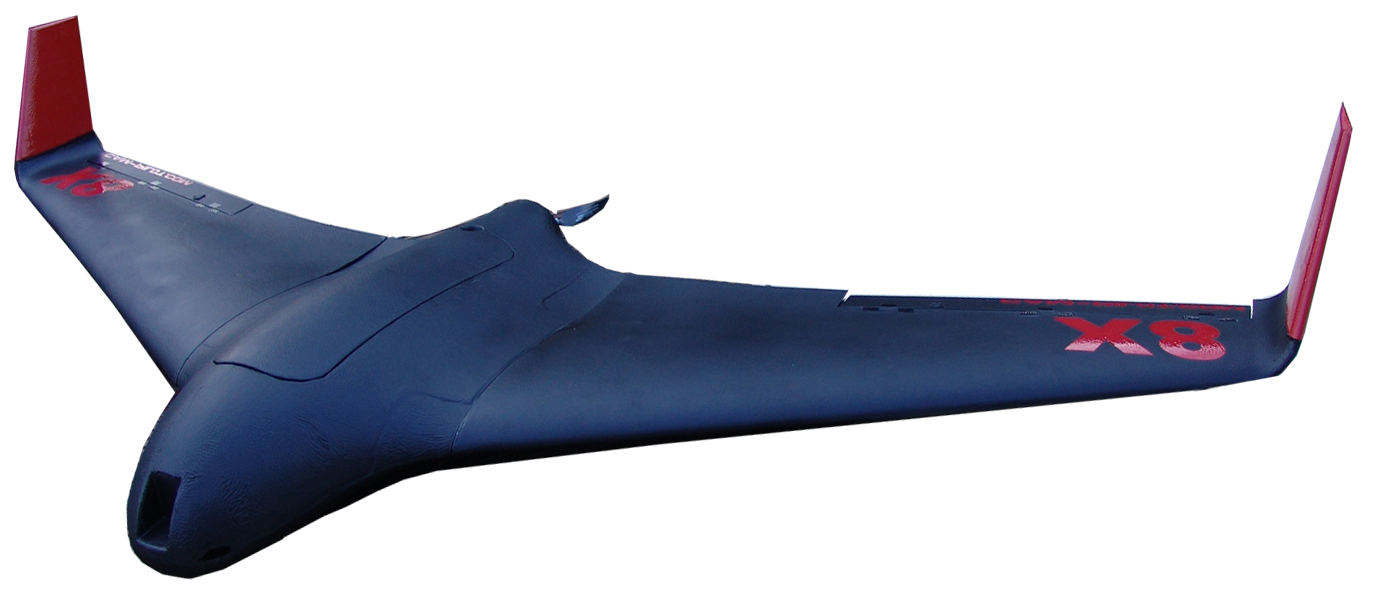
\includegraphics[width=0.7\textwidth]{figs/Wing-X8_white-bgd2.png}
		\caption{X8 Skywalker from Skywalker Technologies, Picture from \url{www.campilot.tv/blog/win-x8}}
		\label{figure:skywalkerX8}
\end{figure}
The X8 has a wingspan of $2120mm$ which allow for a Maximum Take-Off Wight of $4.2kg$, including $1kg$ for the payload. The X8 used in this work is outfitted in according to the specification given in \citep{KlausenX8}. The components that is used in the X8 at the UAVLAB is given in table \ref{tb:X8Components}.
\begin{table}[H]
\begin{center}
\begin{tabular}{l l}
Sensors & 3DR ublox GPS with Compass Kit\\&Pixhawk Airspeed Sensor Kit \\
Servo & Hitec HS-5125MG \\
Motor & Hacker A40 \\
ECU & Jeti Master Spin 66 Pro \\
Main Battery & 1 Zippy Compact 4S 5000 mAh\\
Autopilot & 3DR Pixhawk \\
Primary digital data link & Ubiquiti Rocket M5
\end{tabular}
\end{center}
\caption{Components in the X8 at the UAVLAB}
\label{tb:X8Components}
\end{table}
\subsection{Embedded Computer}
The embedded computer chosen as payload in the X8 is a Beaglebone Black, shown in figure \ref{figure:BeagleBone}. The Beaglebone was chosen because of its sufficient computation power, low energy consumption and variety of communication interfaces. For ease interface access the  the Uavlab at NTNU has developed an extension board called "CAPE".
\begin{figure}[H]
	\centering
		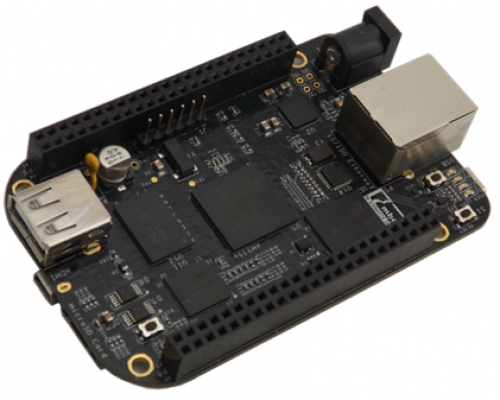
\includegraphics[width=0.7\textwidth]{figs/BeagleBoneBlackE14.png}
		\caption{BeagleBone Black element 14, Picture from \url{http://www.element14.com}}
		\label{figure:BeagleBone}
\end{figure}
The Beaglebone black supports linux operation systems, and it is compatible with the \gls{lsts} toolchain, which will be return to in \ref{S:software}.
\subsection{GNSS receiver}
The system will use two types of \gls{gnss} receivers, namely the Ublox LEA M8T and the Piksi system. 

The Ublox LEA M8T is a new generation of low-cost \gls{gnss} receiver from ublox. The receiver support sending out raw \gls{gnss} data from both \gls{gps} and \gls{glonass} in the same configuration. The receiver have great performance in acquisition and tracking sensitivity of \gls{gnss} satellites. More technical details can be found in  \citep{UbloxDataSheet,UbloxReceiverDescription}.
\begin{figure}[H]
	\centering
		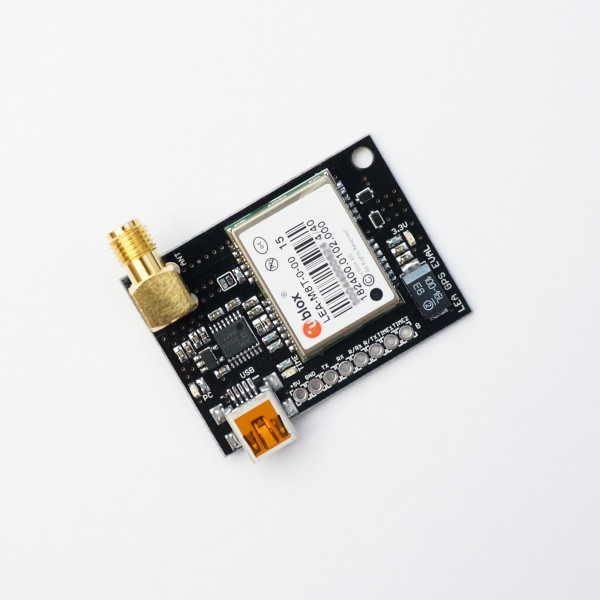
\includegraphics[width=0.7\textwidth]{figs/ubloxLeaM8T.jpg}
		\caption{Ublox LEA M8T, Picture from \url{http://www.csgshop.com}}
		\label{figure:Ublox}
\end{figure}
\subsubsection{Piksi}\label{ss:Piksi}
The Piksi system is a low cost, high performance \gls{gps} receiver with \gls{rtk-gps} functionality with capability for centimeter level relative positioning accuracy developed by Swift Navigation, shown in figure \ref{figure:Piksi}. Piksi is ideal for autonomous vehicles because of its small form factor, fast position solution update rate and low power consumption. 
More detailed information about Piksi can be found in \citep{Piksiv231}
\begin{figure}[H]
	\centering
		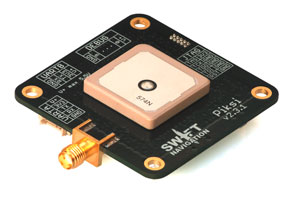
\includegraphics[width=0.7\textwidth]{figs/piksi_top.jpg}
		\caption{Piksi receiver, Picture from \url{www.swiftnav.com}}
		\label{figure:Piksi}
\end{figure}
The communication structure for Piksi used in this project work is seen in figure \ref{figure:CommunicationPiksi}.
\begin{figure}[H]
	\centering
		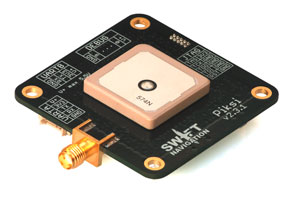
\includegraphics[width=0.7\textwidth]{figs/piksi_top.jpg}
		\caption{Communication structure for Piksi}
		\label{figure:CommunicationPiksi}
\end{figure}
\subsection{GNSS Antenna}
The navigation system will use two \gls{gnss} antenna, one for the \gls{uav} and the other for the base station. The main criteria for the \gls{uav} antenna is that it's small,compact and have a light weight.

The M1227HTC-A-SMA, seen in figure \ref{figure:Maxtena} has been used in other \gls{uav} setups at the UAVLAB with good results. The antenna is small, compact and with an light weight of $17g$. It's design for L1/L2 gps/glonass bands. Further information or specification can be found in the datasheet \citep{maxtena}

The base station do not have any restriction on size, weight or aerodynamic. The important factor for a base station antenna is that it has good multipath rejection. Also the base station position should be calculated as accurate as possible which impose further restriction on interference handling, phase center stability and noise rejection.

The Novatel GPS-701-GG, seen i figure \ref{figure:Novatel}, was chosen as the base station antenna. The antenna has excellent multipath rejection whit a highly stable phase center. It has reception for both \gls{gps} and \gls{glonass} \gls{l1} signals.Further information or specification can be found in the datasheet \citep{novatel}.

\begin{figure}[H]
	\centering
		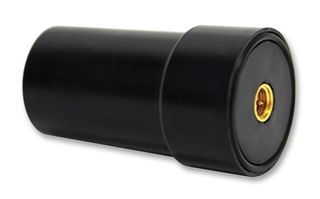
\includegraphics[width=0.7\textwidth]{figs/Maxtena-M1227HCT-A-SMA-image.jpg}
		\caption{The rover \gls{gnss} antenna, Picture from \url{http://sigma.octopart.com/21411362/image/Maxtena-M1227HCT-A-SMA.jpg}}
		\label{figure:Maxtena}
\end{figure}

\begin{figure}[H]
	\centering
		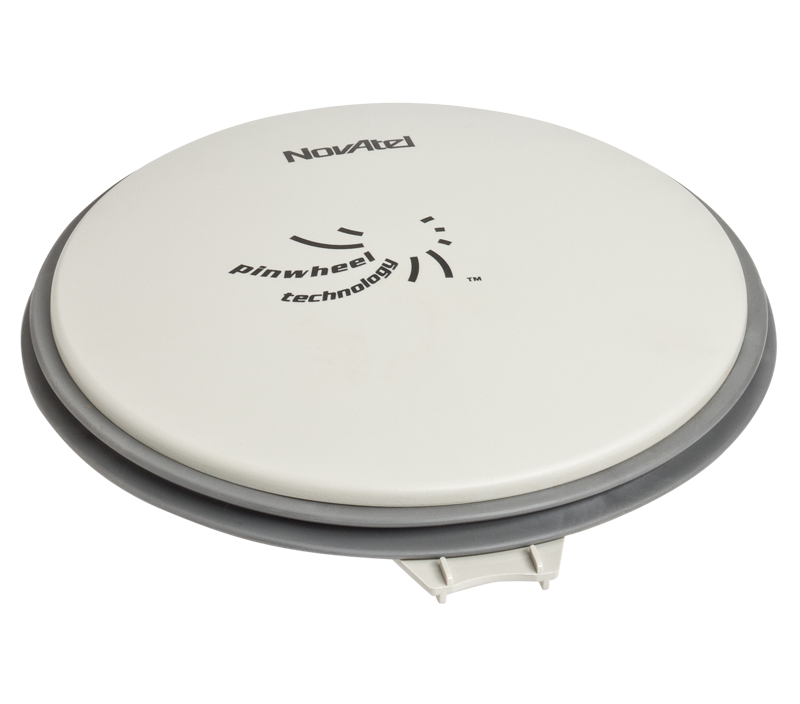
\includegraphics[width=0.7\textwidth]{figs/702-L.png}
		\caption{The base station \gls{gnss} antenna, Picture from \url{http://www.novatel.com}}
		\label{figure:Novatel}
\end{figure}


\section{Software}\label{S:software}
This section contain the different software that is used in the X8 system. The following sections contain the operating system that runs on the base station and rover, the middleware used to perform the different tasks, the messages protocol, the missionplaner program and rtklib which will have the main focus.
\subsection{LSTS toolchain}
The Laboratório de Sistemas e Tecnologia Subaquática (LSTS) toolchain is used a platform for software implementation. This is a flexible, scalable, open-source software that supports integration and control of various types of unmanned vehicles \citep{pinto2013lsts}. The toolchain includes a operating system, runtime environment, message protocol and a command and control for operations. The following program is included in the toolchain
\subsubsection{GLUED}
Glued is a minimal Linux operating system distribution, and design with embedded system in mind. It is platform independent, easy to configure and contain only the necessary packages to run on a embedded system. This makes GLUED a light and fast distribution. GLUED is configured through a single configuration file that which can be created for a specific system. 
\subsubsection{Dune}
Dune (DUNE Uniform Navigation Environment) is a runtime environment for unmanned systems. DUNE is operating system independent and can run on-board the embedded computer. It can interact with the sensors, actuators and payload. It can also be used for tasks like communication, navigation, control, manoeuvring, plan execution and supervision.

Dune works by setting up individual task that can dispatch and subscribe to different \gls{imc} messages.
\subsubsection{IMC}\label{ss:IMC}
The \acrfull{imc} protocol is build to interconnect systems of vehicles,sensors and human operators. The protocol is a messages-oriented protocol that enable exchange of real-time information about the environment and updated objectives, such that the participant in the communication can pursue a common goal cooperatively.
\gls{imc} has a standard way of dispatching and consuming messages, which abstracts hardware configuration from the software. All \gls{imc} messages are logged by DUNE.

%Other feature: Not assuming a specific software architecture, can generate native support for different programming languages and/or computer architectures. Used in network nodes, inter-process and inter thread communication
\subsubsection{Neptus}
Neptus is an open source command and control software that can be used for a single or fleet of unmanned vehicles with different types of sensors. The operator can observe real time data from a vehicle, review previous missions and plan future mission. In this work Neptus has been used to extract data logged by Dune during a defined mission, and to monitor the integer ambiguity solution from \gls{rtklib} and Piksi.
\subsection{RTKLIB}\label{ss:Rtklib}
\acrfull{rtklib} is a open source program package for standard and precise positioning with GNSS developed by T. Takasu. \gls{rtklib} can use raw GNSS data to estimate the position of the rover. \gls{rtklib} can be configured to give a position solution in real time in differential mode. Figure \ref{figure:RTKLIB_STRUCTURE} shows how \gls{rtklib} can be used in a RTKGNSS mode. The two main moduels here is str2str and rtkrcv. Both will be explained more closely in the following sections. More information about  \gls{rtklib} can be found in \citep{Rtklib242}.

\begin{figure}[H]
	\centering
		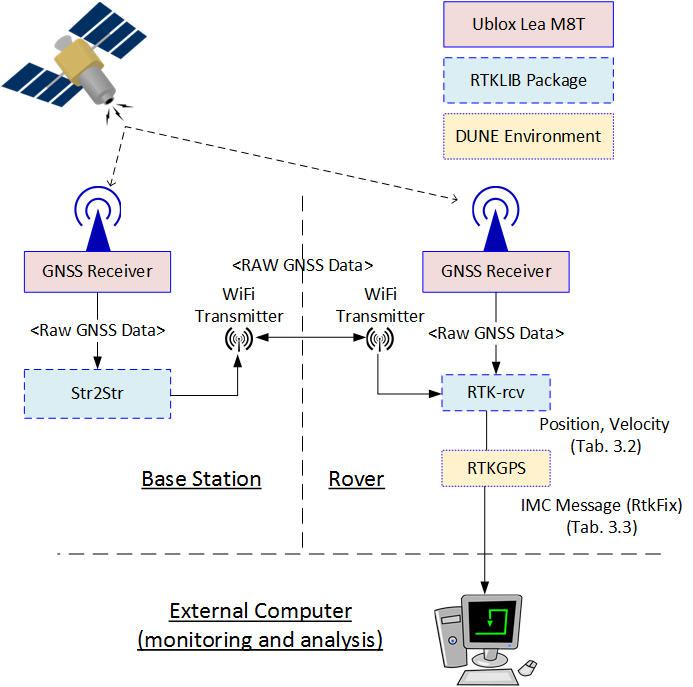
\includegraphics[width=0.7\textwidth]{figs/RTKLIB.png}
		\caption{The communication structure of \gls{rtklib}}
		\label{figure:RTKLIB_STRUCTURE}
\end{figure}
\subsubsection{Rtkrcv}
As part of the \gls{rtklib} Rtkrcv is  used to calculate the position of the rover in real time.
Rtkrcv can be configured to have two output streams. The structure of the output stream is given the \gls{rtklib} manual\citep{Rtklib242}. It's desired in a automatic landing system that have that velocity solution. This is was not provided in the newest version of \gls{rtklib}, and therefore the source code was altered to send out the velocity data. The position output is in \gls{enu} format and the full output structure is shown in table \ref{Tb:RtklibOutput}
\begin{table}[H]
\begin{center}
    \begin{tabular}{ | l | l |}
    \hline
    \textbf{Header} & \textbf{Content} \\ \hline
     1 Time & The epoch time of the solution indicate the true receiver\\& signal reception time. Can have the following format:\\&\\& yyyy/mm/dd HH:MM:SS.SSS:\\& Calender time in GPST, UTC or JST.\\&\\&
     
     WWWW SSSSSSS.SSS:\\&
     GPS week and TOW in seconds  \\ \hline
     2 Receiver Position & The rover receive antenna position \\ \hline
     3 Quality flag (Q) & The flag which indicates the solution quality.\\& 1:Fixed\\& 2:Float\\& 5:Single \\ \hline
     4 Number of valid satellites (ns) & The number of valid satellites for solution estimation. \\ \hline
     5 Standard deviation & The estimated standard deviation of the\\& solution assuming a priori error model and error\\& parameters by the positioning options \\ \hline
     6 Age of differential & The time difference between the observation data epochs\\& of the rover receiver and base station in second. \\ \hline
     7 Ratio factor & The ratio factor of "ratio-test" for standard integer\\& ambiguity validation strategy \\ \hline
     8 Receiver velocity & The velocity of the rover. Given only when output is\\& in enu format \\ \hline
    \end{tabular}
\end{center}
\caption{Rtklib output solution format }
\label{Tb:RtklibOutput}
\end{table}
When set configured as a differential GPS rtkrcv uses the \gls{lambda} method to resolve the integer ambiguity., which is further explained in \citep{LAMBDAMETHOD}. The solution is considered fixed if the ration between the best estimate and the second best estimate is above a certain threshold.

The position solution is calculated with a Extended Kalman Filter, that can have different structure depending on how rtkrcv is configured
\subsubsection{Str2str}
Str2str is used as a base station program that can retrieve raw \gls{gnss} data and create a tcp sever, which the rtkrcv program can connect itself as a client. Str2str sends out RMTC3 formatted messages, however it can be configured to send whatever comes in as input.
\section{Implementation}
This section explain how the \gls{rtk-gps} navigation system has been implemented in the \gls{uav} system used in the testing. The implementation includes both a software and a hardware part, as shown i figure \ref{figure:HardSoft}.

\begin{figure}[H]
	\centering
		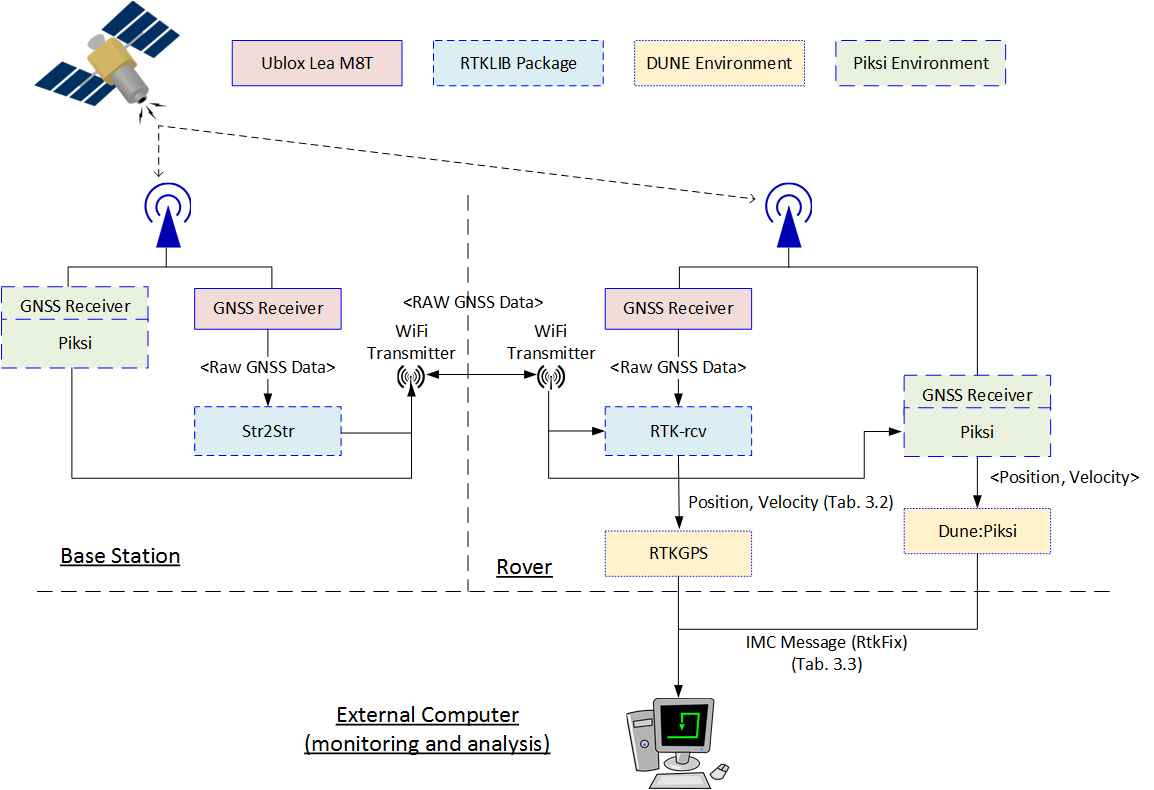
\includegraphics[width=0.7\textwidth]{figs/Combined.png}
		\caption{Hardware Software interaction}
		\label{figure:HardSoft}
\end{figure}
\subsection{Software implementation}
The software implemented is shown in figure \ref{figure:HardSoft}, where the different modules are available from the UAVLAB. The detailed implementation has been trough configuration of the config files, including alteration of the existing implementation.
\subsubsection{RTKGPS}
The \gls{rtk-gps} module in the navigation system includes \gls{rtklib}, and the two Dune tasks RTKGPS and Piksi. The RTKGPS task is connected to \gls{rtklib} though a virtual connection, and the Piksi task has a physical connection to the Piksi receiver, as shown i figure \ref{figure:HardSoft}.


\gls{rtklib} is implemented into the base station and the rover. The base station implementation use the  str2str program to communicate with the Ublox over a uart cable, outputs raw \gls{gnss} data over tcp to the rover.
The rover uses the rtkrcv program from \gls{rtklib} to estimate the position of the rover. Rtkrcv receive raw \gls{gnss} data from both the str2str program and the Ublox installed in the \gls{uav}, as shown in figure \ref{figure:RTKLIB_STRUCTURE}. Rtkrcv is configured in a moving baseline configuration to simulate the behaviour that is expected during a landing on a ship. The configuration file is included in \ref{APPENDIX:RTKLIB}.

The output from the RTKGPS task is a \gls{imc} message called RtkFix, see table \ref{Tb:RtkFix}, which include the relative position of the \gls{uav} as well as the velocity, type of integer solution and the \gls{gps} \acrfull{tow}. The \gls{imc} message is further sent to an external computer for monitoring over TCP/IP (Wifi).
\begin{table}[!h]
\begin{center}
    \begin{tabular}{ | l | l |}
    \hline
    \textbf{Header} & \textbf{Content} \\ \hline
     tow & Gps time of Week  \\ \hline
     n & Baseline North coordinate \\ \hline
     e & Baseline East coordinate \\ \hline
     d & Baseline Down coordinate \\ \hline
     v\verb=_=n & Velocity North coordinate \\ \hline
     v\verb=_=e & Velocity East coordinate \\ \hline
     v\verb=_=d & Velocity Down coordinate \\ \hline
     iar\verb=_=hyp & Number of hypotheses in the Integer Ambiguity Resolution \\ \hline
     iar\verb=_=ratio & Quality ratio of Integer Ambiguity Resolution \\ \hline
     type & Type of fix: \\& None = No solution, but RTK task is running
     \\& Obs = No solution, but receiving observations
     \\& Float = Floating point solution of Integer Ambiguity Resolution
     \\& Fix = Fixed(single) solution of Integer Ambiguity Resolution \\ \hline
    \end{tabular}
\end{center}
\caption{The \gls{imc} message RtkFix }
\label{Tb:RtkFix}
\end{table}

\subsection{Hardware implementation}
Both the base station and \gls{uav} has been fitted with a \gls{gps} antenna splitter, seen i figure \ref{figure:AntennaSplitter}, such that both receivers receive the same signals from the antennas. GLUED is used as the operating system in the Beaglebone on both the base station and the \gls{uav}. The Piksi and Ublox is connected with the Beaglebone over uart cables. The primary data-link between the \gls{uav} and the base station with Ubiquiti AirMax radios.
The embedded computer uses GLUED as its operating system, and on it runs both Dune and \gls{rtklib}. The Piksi and Ublox is connected to the BeagleBone over uart cables.
More information on the hardware setup used in the X8 and the Base station is given in \citep{KlausenX8}
\begin{figure}[H]
	\centering
		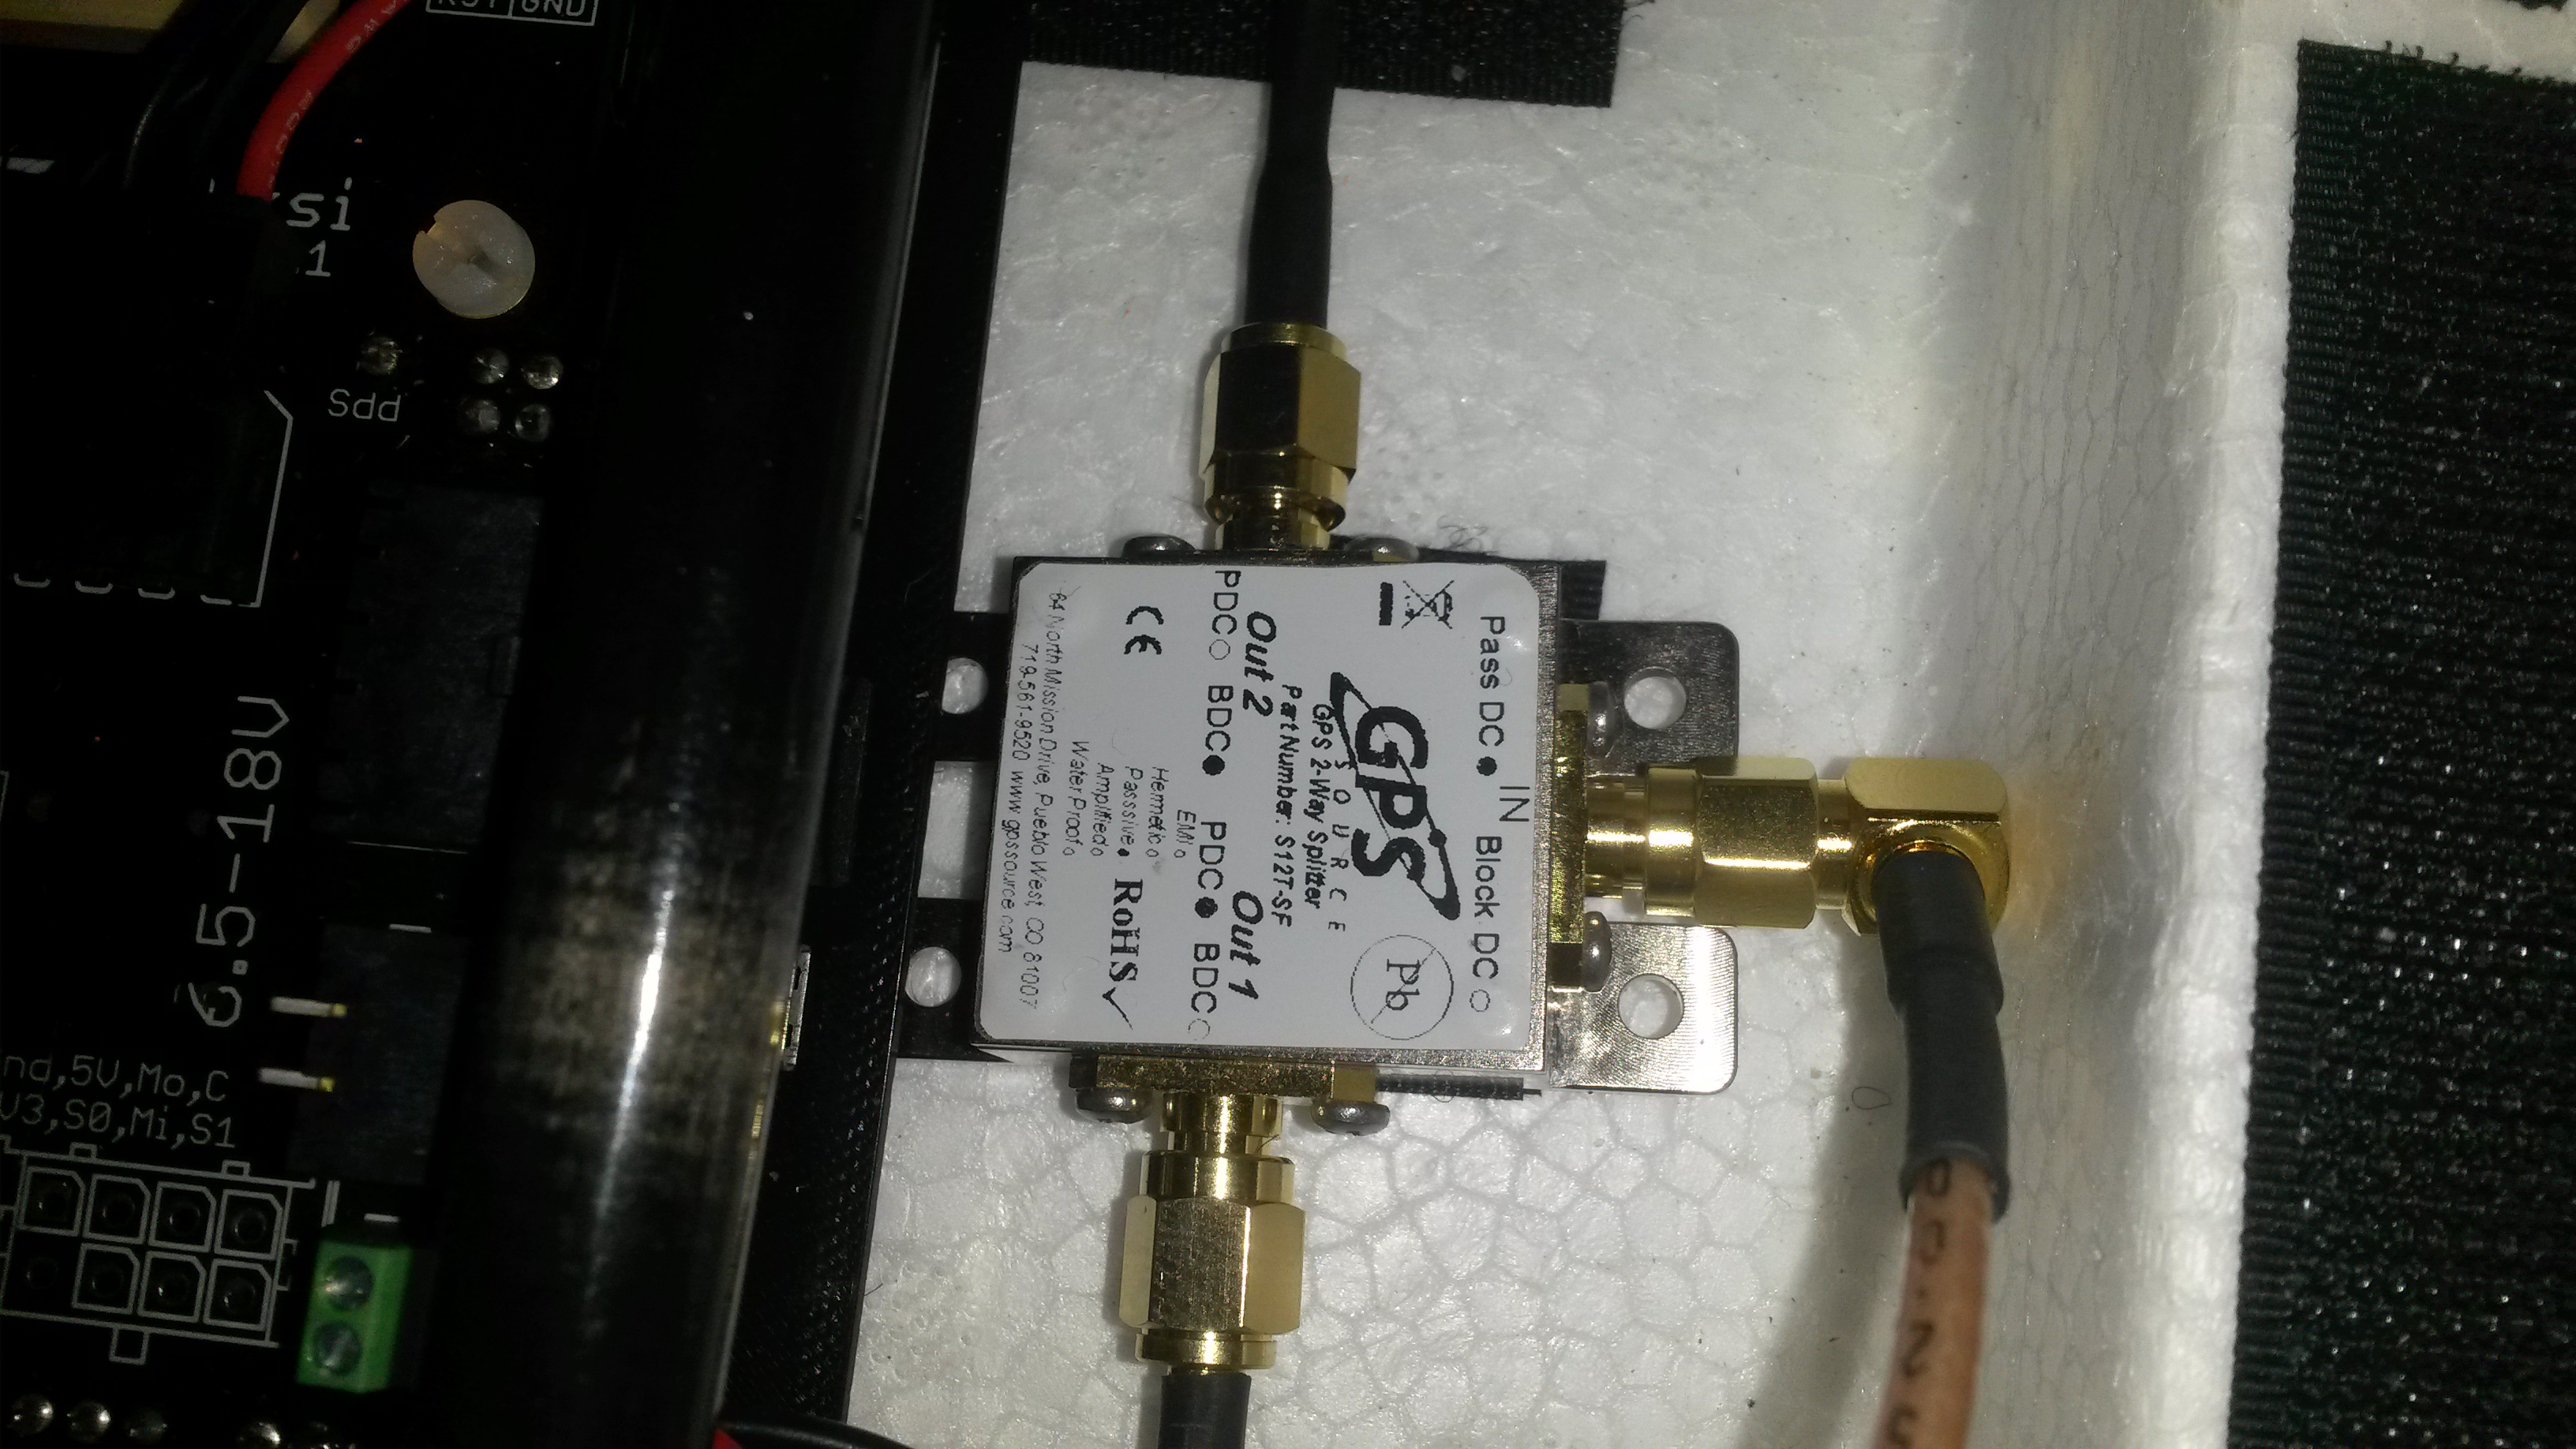
\includegraphics[width=0.7\textwidth]{figs/066.jpg}
		\caption{\gls{gps} antenna splitter}
		\label{figure:AntennaSplitter}
\end{figure}
\cleardoublepage
\chapter{Implementation}
The chapter will explain how the different software are connected and what information is sent between them. All the configuration and start up commands can be found in the appendix.
\section{Software implementation}
The software implementation consist mainly of rtklib and dune. Piksi is also used in the experiment, however it's rtklib and the Dune task RTKGPS that will be discussed thoroughly.
\subsection{Rtklib}
Rtklib is sepperated into the base station and the rover. The base station implementation runs the app str2str were it communicate with the ublox over a uart cable, and start up a tcp server.

The rover uses the rtkrcv app from rtklib to estimate the position of the rover. Rtkrcv connect itself as a tcp client to the tcp server that str2str create. Rtkrcv is configured in a moving baseline configuration to simulate the behavior that is expected during a landing on a ship. (Referer her til teori kap om rtklib)

Rtkrcv output the solution data over a virtual uart connection that is created by a program called socat. The output structure is given i (se rtklib com kap)
\subsection{Rtkgps}
Rtkgps is a task in Dune that takes the output from rtklib and create a rtkfix imc message that is dispatch into the Dune/Neptus network. Rtkgps consists of two parts. One reads the message from the virtual uart, and the other create and dispatch the rtkfix imc message.

\subsection{Neptus}
Neptus is used as interface for the human operator, and for after mission reviews. In this thesis it's only used for after mission reviews, however it has the cabillity to give a landing command to the rover (henvis her til frølich)
PLASSERES I APPENDIX
\subsubsection{str2str configuration}
The system has to instances of rtklib. The base station uses the str2str and the x8 uses rtkrcv. str2str is configured to receive raw data from the ublox at a frequency of 10 Hz. The connection between str2str and the GNSS receiver is a uart cable that is configured with a baudrate at 115200. The program starts a tcp serve were rtkrcv becommes a client.

Very short about how Glued is used: Start up, 

About rtklib: What does rtklib do in the system, were do it run, what instances is used, how do it connect to dune, what is the output message

About dune: What task are used to communicate with rtklib, how do they communicate, what is the output of the given task

About Neptus: What do neptus do, how is it used in the system, how will it be used in a automatic landing senario.

About Ardupilot: Very short on what Ardupilot do in the system 



All in one section unless something need more space.
Write here how rtklib is configured and how the system is connected
Write here how Dune receive data from rtklib and what task is used. Include also what imc message is involeved in the task
Write here how neptus is configured for the test, and how it is used
How Glued is configured to run rtklib and Dune
\section{Hardware implementation}
The embedded computer uses GLUED as its operating system, and on it runs both Dune and rtklib. The Piksi and Ublox is connected to the BeagleBone over uart cables.

TRENGER SYSTEM FIGUR SOM VISER HVORDAN UAV ER FORBUNDET MED BASE
The two \gls{rtk-gps} system is connected to a antenna splitter , figure \ref{figure:AntennaSplitter}, such that both system receive the same \gls{gnss} signals.

\begin{figure}[H]
	\centering
		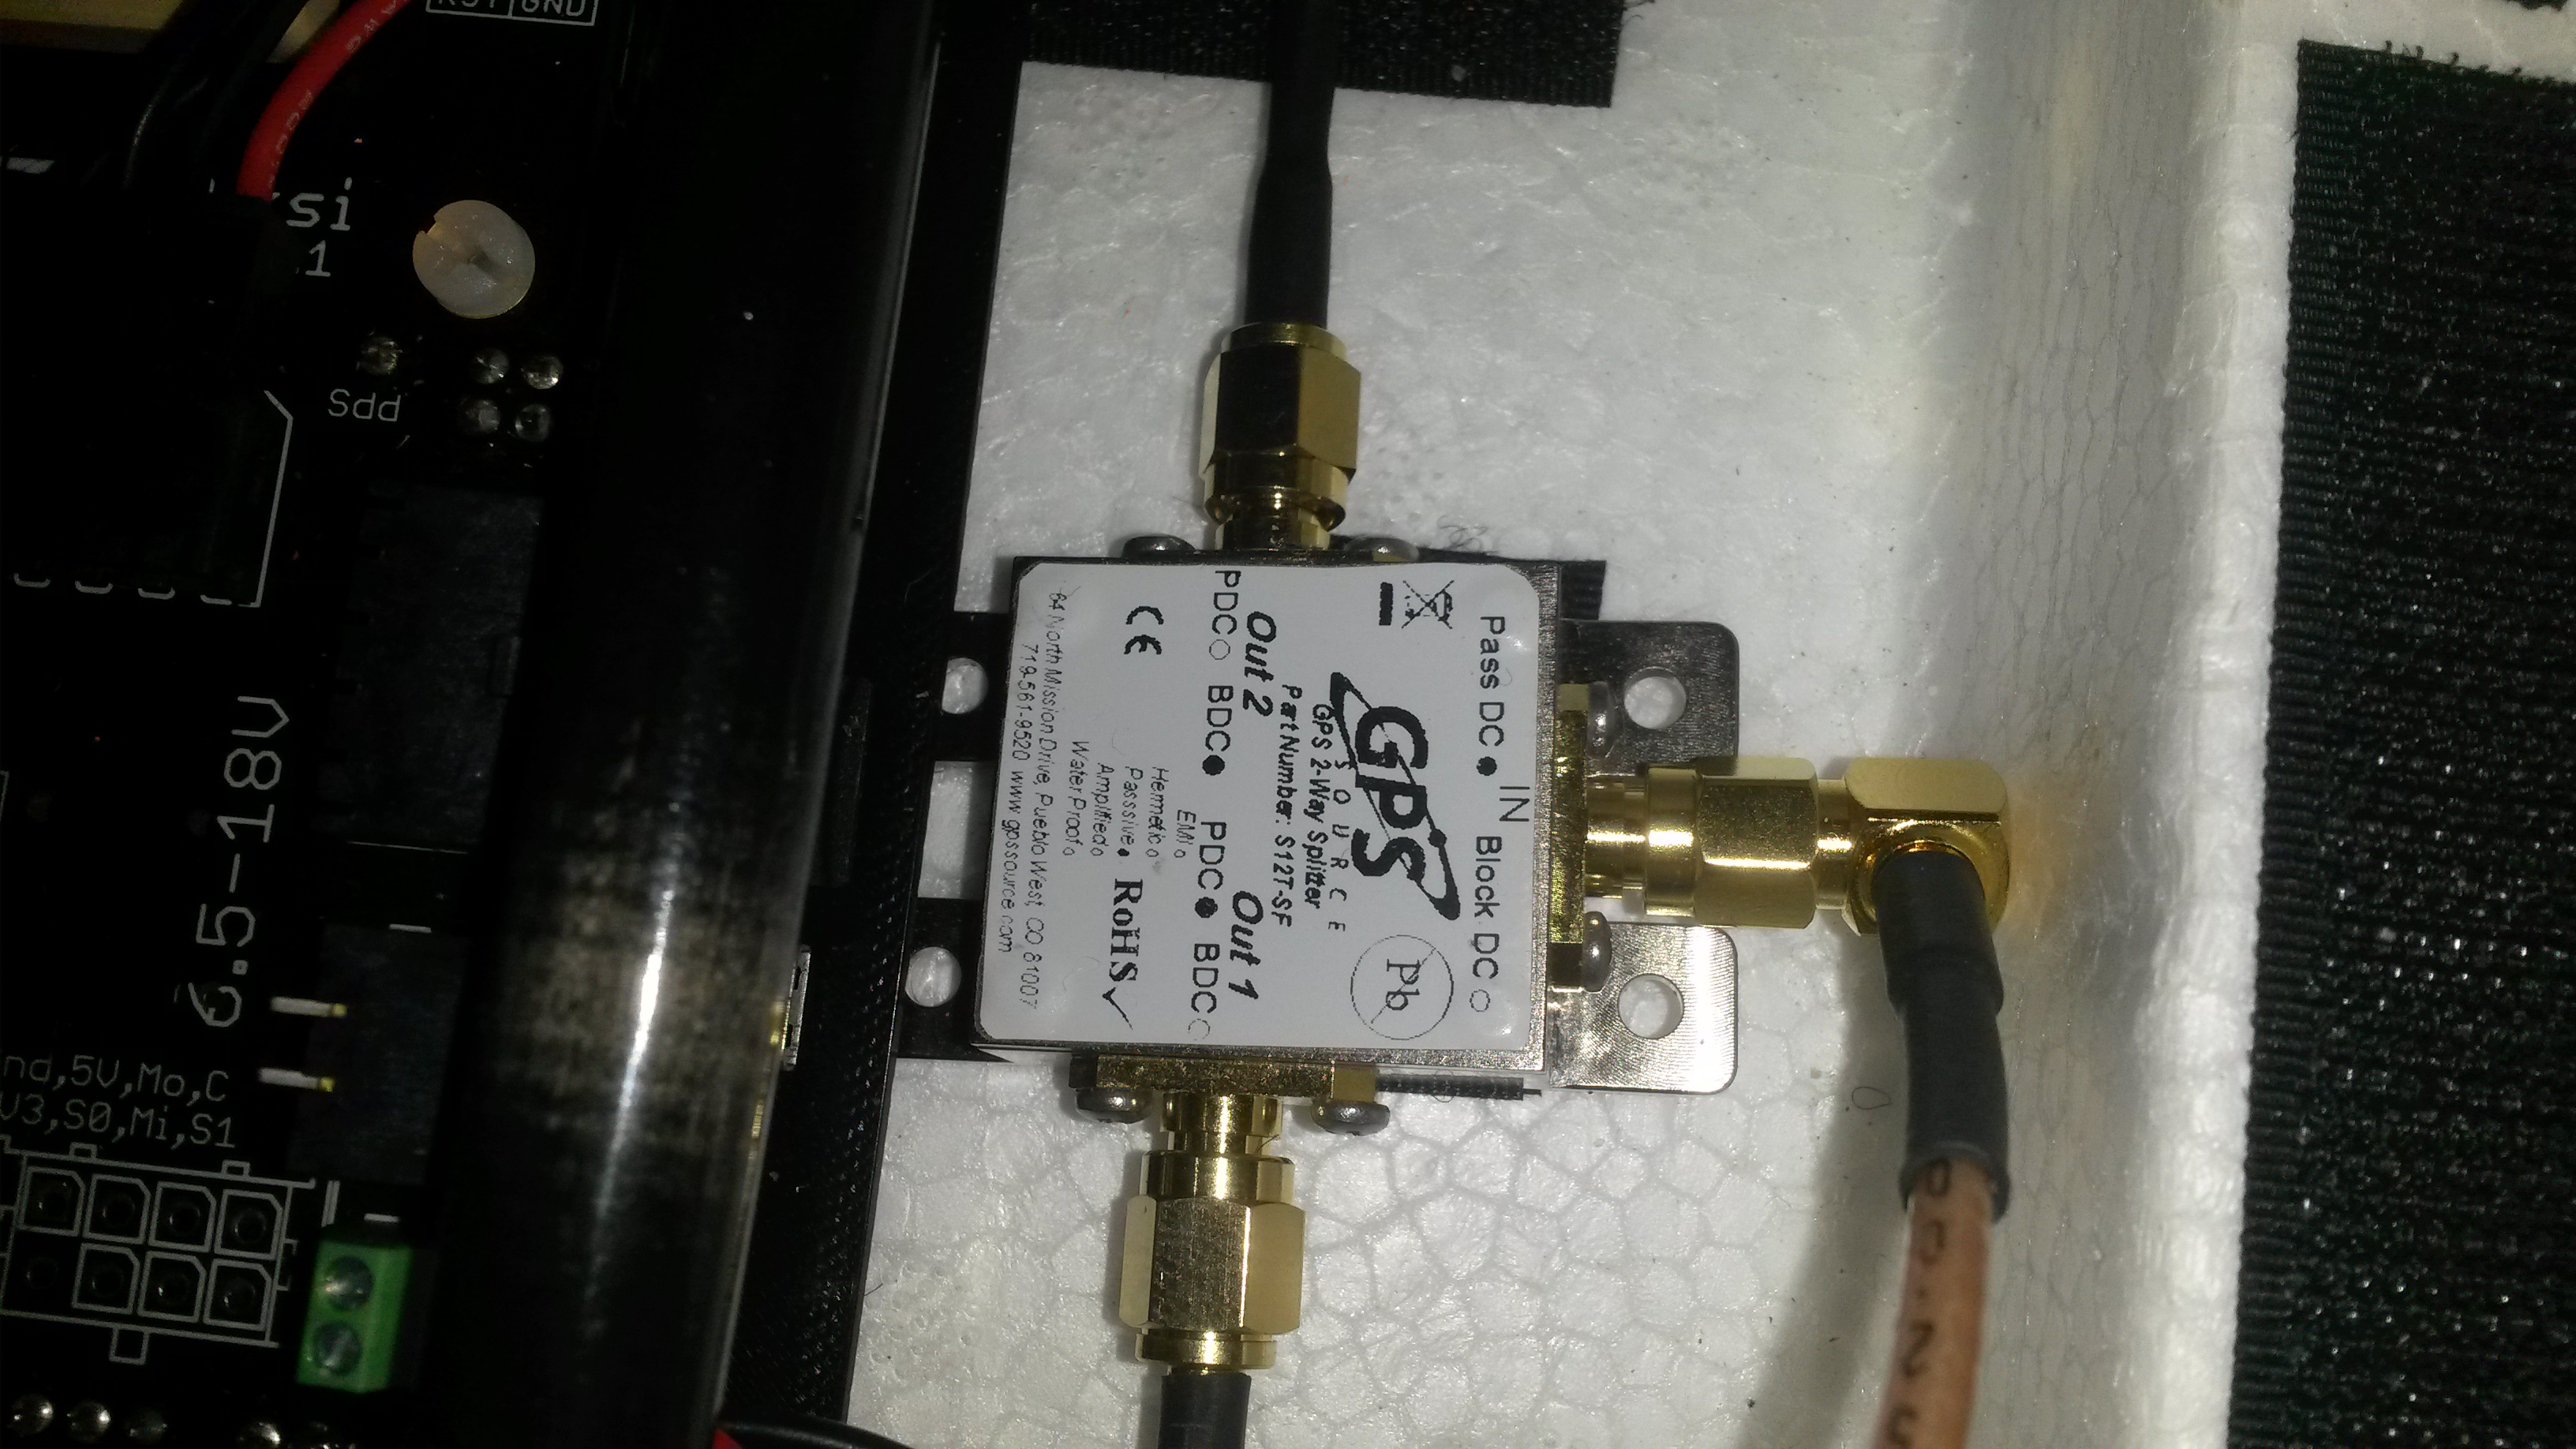
\includegraphics[width=0.7\textwidth]{figs/066.jpg}
		\caption{Antenna splitter}
		\label{figure:AntennaSplitter}
\end{figure}

This section contain how all the physical components are connected at both the rover and the base station. Include also how everything was prepared.

About Beaglebone: What runs on the beaglebone, connections, devices, what is it place in the system

About Ublox: Explain the ublox from a system perspective, how it's connected

Pixhawk: What do it do in the system:

Piksi: Same as ublox

The X8: How do it fit in the system

The base station: Same as x8

Antennas: 

Wifi router


%===================================== CHAP 5 =================================

\chapter{Experimental testing}
This chapter contain the result from the test that were performed. The goal with these test was to evaulate the ublox receiver againgst the pixi receiver, and to get a impresion on the accuracy to the rtklib solution with ublox. The comparison test was performed with the pixi and ublox connected to the same antenna at both the rover and the base station. Then the deviation in the position estimate can only come from the receivers. The accuracy test of the ublox was tested by performing the same manoeuvre several times. All position and velocity data is given in the \gls{ned} frame. 
\section{Physical testing}
The experimental test was split in two independent test, one where the X8 \gls{uav} was carried around on a open field to test the performance of the \gls{rtk-gps} system in a more controlled environment. The goal of the first was to log data from both \gls{rtk-gps} system in optimal condition for the navigation system. The second test was perform in a more realistic environment for a navigation system. 


\subsection{Test 1: Test of the RTK-GPS navigation system}
In this part two sessions of navigation data will be presented. Both sessions were performed on the same day, which was cloudless and at a time with low \gls{dop}. The raw data from the Ublox receiver was post processed with rtklib, and is should be more accurate than it's real time counter part. Therefore a error was defined as:
\begin{equation}
e(t) = p_r(t) - p_p(t)
\end{equation}
where $p_r(t)$ and $p_p(t)$ is defined as the position solution from the real time system and the position solution from the post processed solution respectfully. It should be noted that in order to compare the different time-series the position data was synchronized with each other. From the error the cumulative standard deviation for the error was calculated using the matlab function "std".
\subsubsection{First session}
As expected both systems provided a position estimate with fixed integer solution that followed the true path, and further confirms that both system performed in a similar manner. Therefore both systems are suitable for further comparison of position estimation in a flying test.
Figure \ref{figure:xywalk1} shows a North East plot of how the walk was. The plot contain only the fixed solution from both the piksi and rtklib. 
\begin{figure}[H]
	\centering
		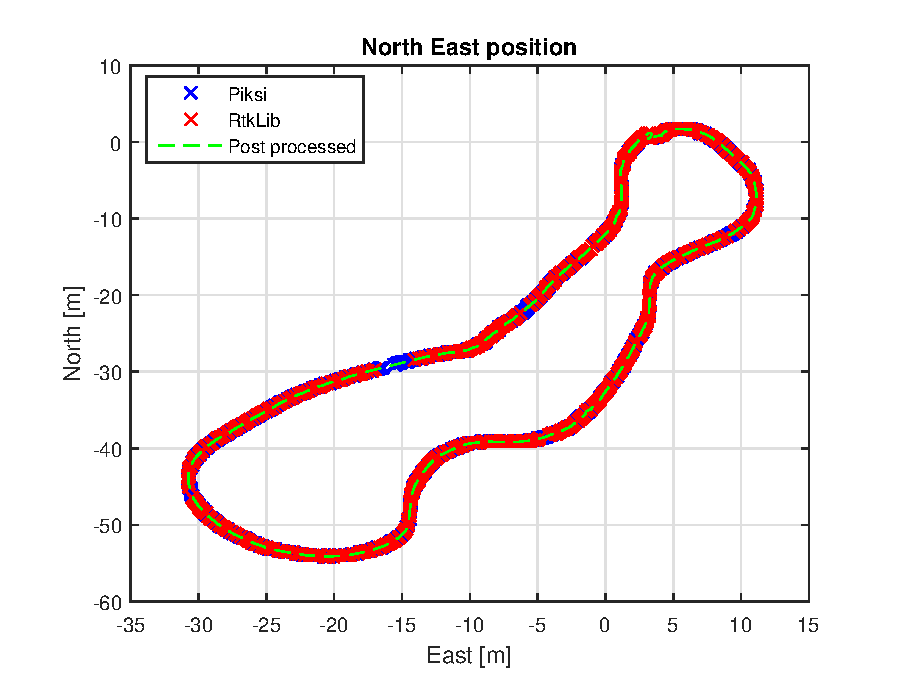
\includegraphics[width=0.7\textwidth]{figs/plots/xywalk1.eps}
		\caption{A xy plot of the piksi,rtklib real time solution and the rtklib post processed solution}
		\label{figure:xywalk1}
\end{figure}
Figure \ref{figure:DownAndAmbwalk1} shows the down position, as well as how the integer ambiguity solution was during the experiment. As seen in the figure both the Piksi and Rtklib manage to keep there fixed solution. The position solution from both the Piksi and Rtklib agrees with the post processed solution. 
\begin{figure}[H]
	\centering
		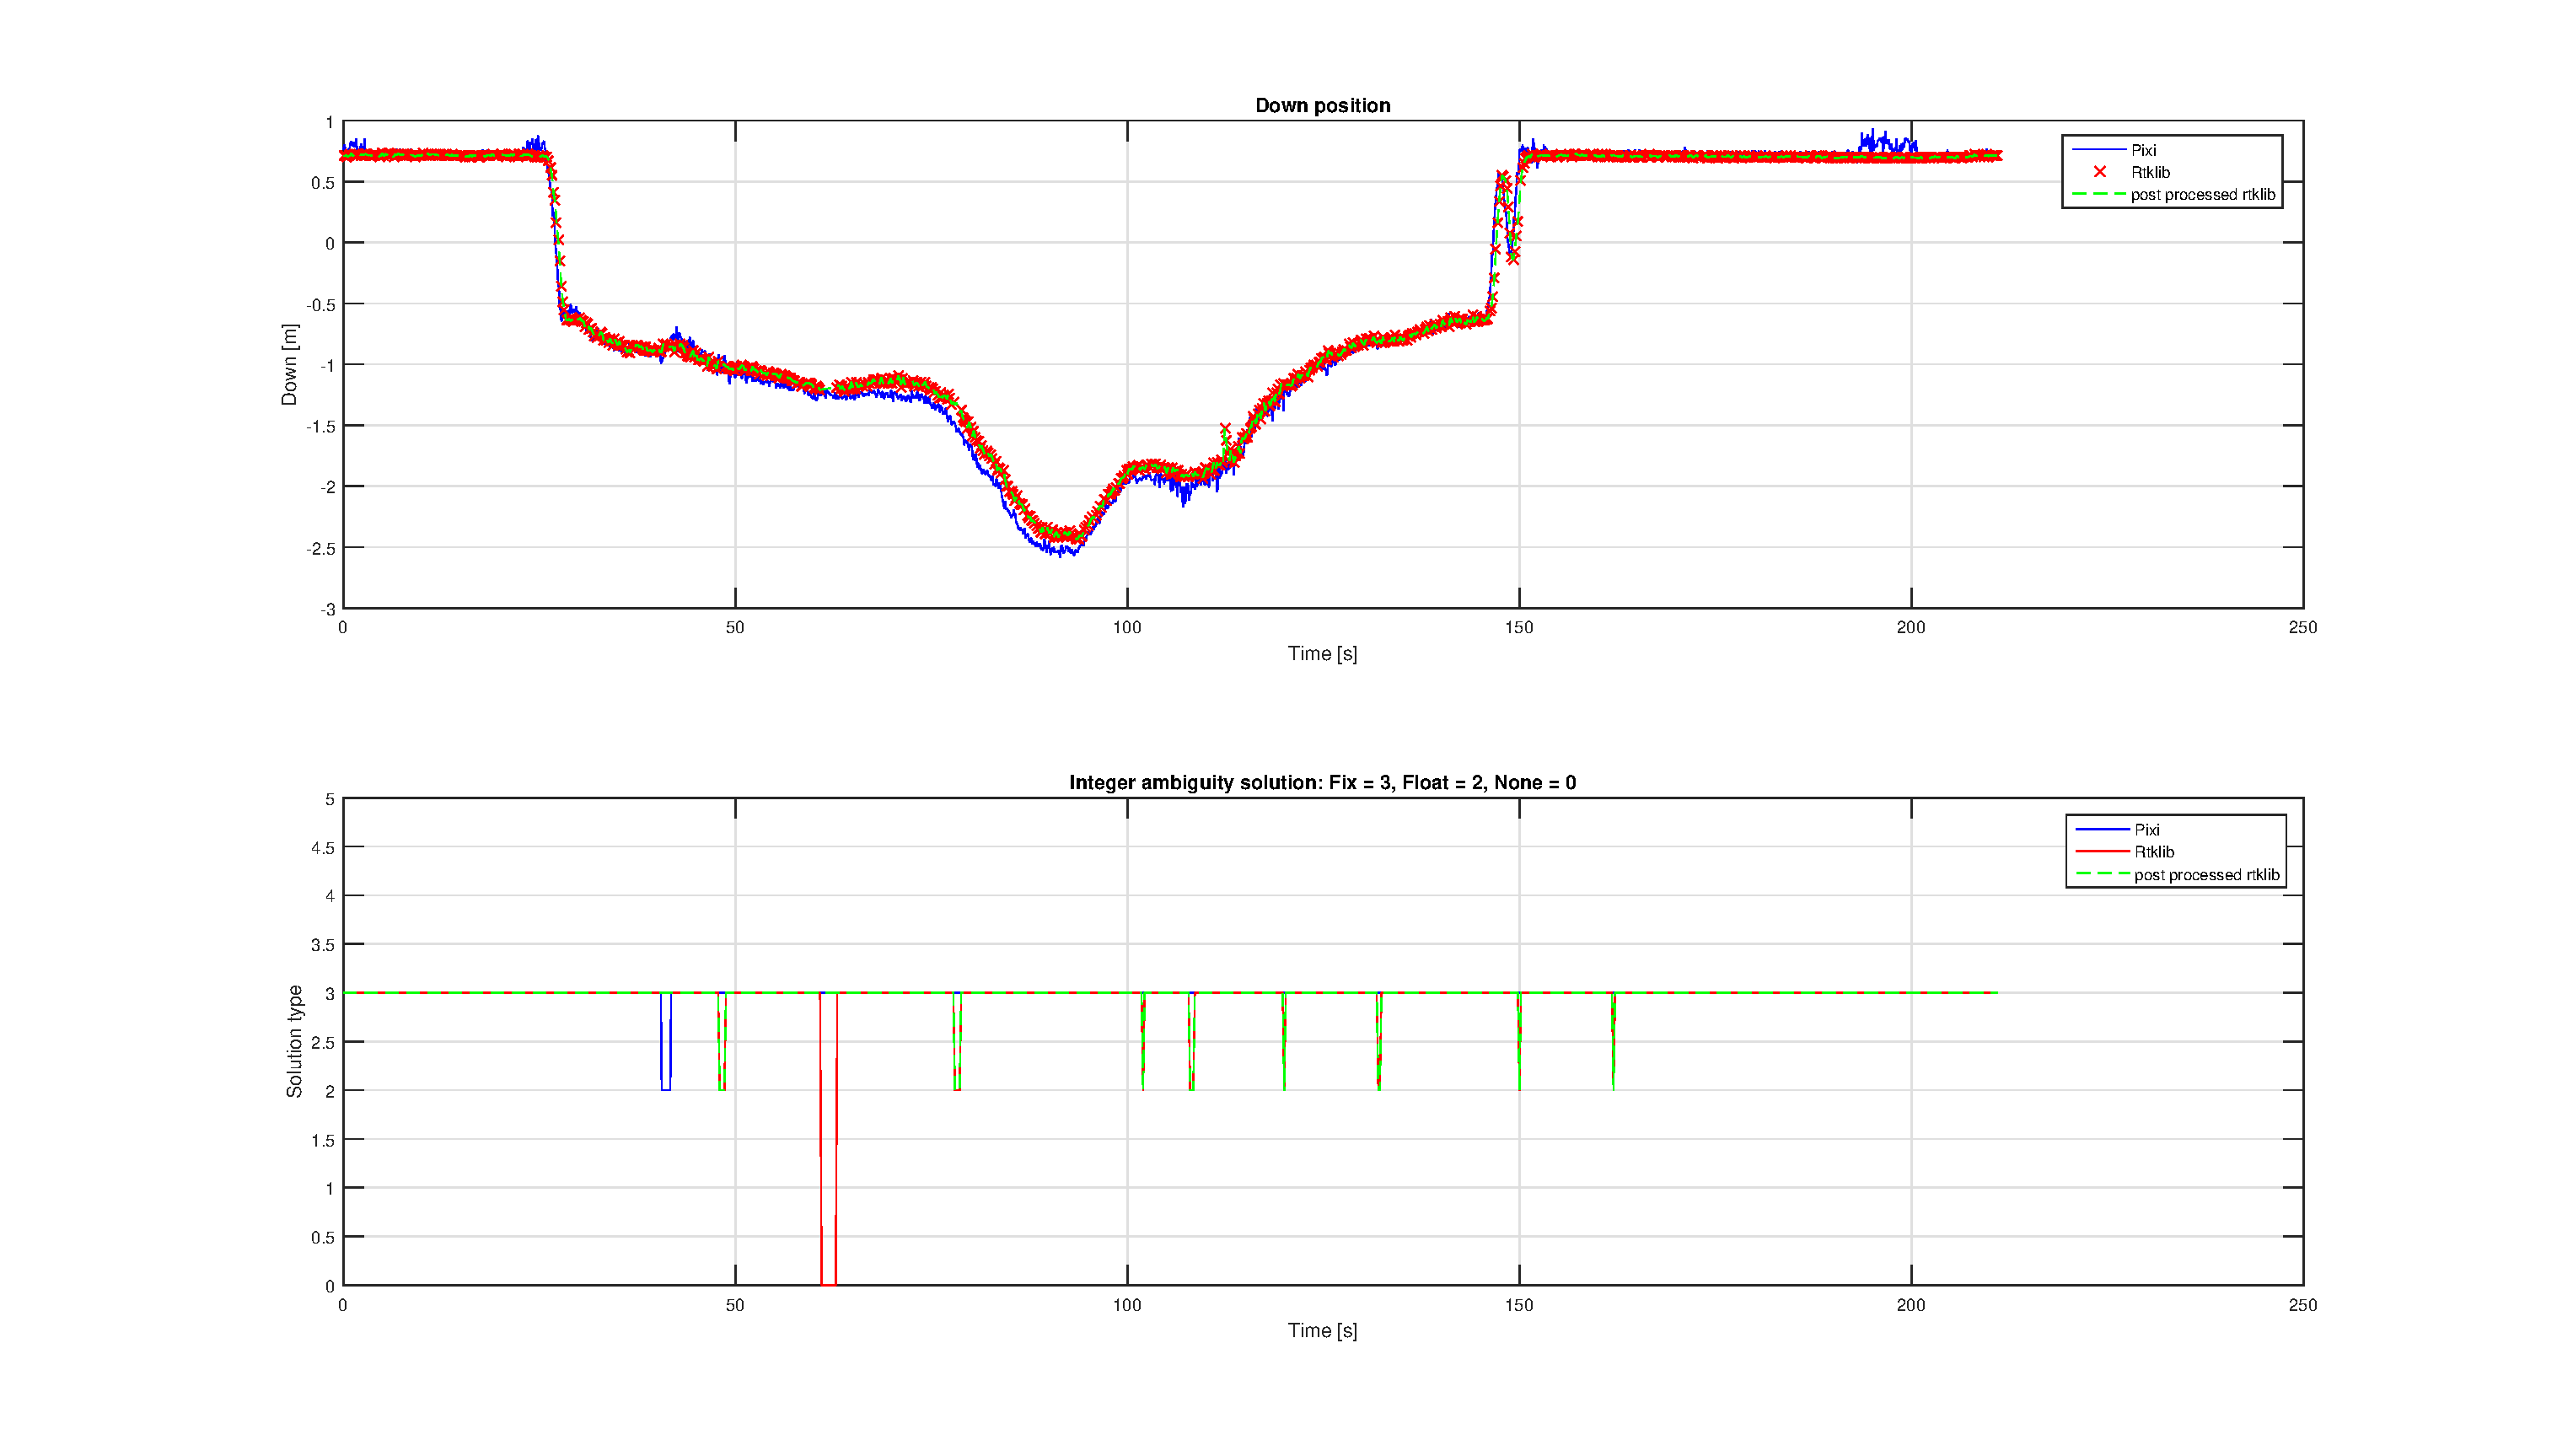
\includegraphics[width=0.7\textwidth]{figs/plots/downWalk1.eps}
		\caption{The communication structure of rtklib}
		\label{figure:DownAndAmbwalk1}
\end{figure}

As seen in figure \ref{figure:xywalk1} the difference between the different solution appear to be small, which is comfirmed in the error plot shown in figure \ref{figure:errorRTKwalk1} and \ref{figure:errorPiksiwalk1}
\begin{figure}[H]
	\centering
		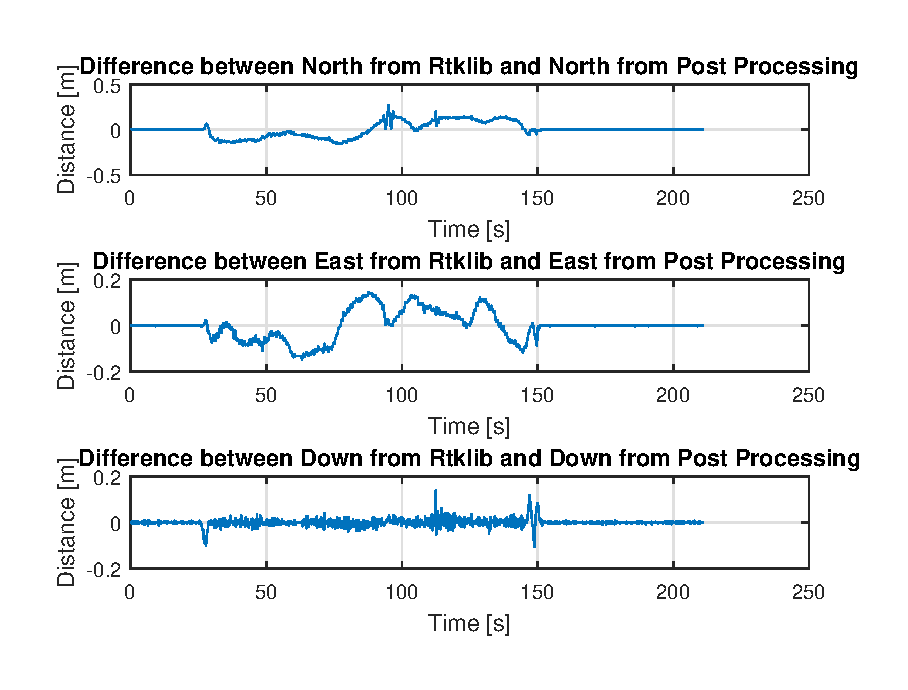
\includegraphics[width=0.7\textwidth]{figs/plots/ertkpost.eps}
		\caption{The difference between rtklib real time and post processed solution}
		\label{figure:errorRTKwalk1}
\end{figure}
\begin{figure}[H]
	\centering
		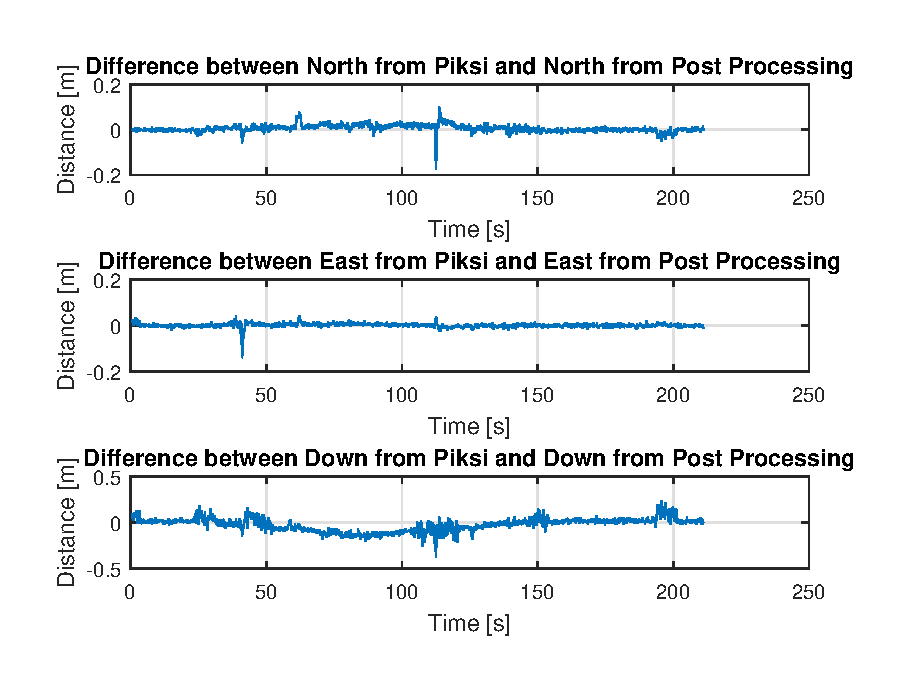
\includegraphics[width=0.7\textwidth]{figs/plots/epiksiport.eps}
		\caption{The communication structure of rtklib}
		\label{figure:errorPiksiwalk1}
\end{figure}
The small variasion in the position error can be seen in figure \ref{figure:stdPiksi} and \ref{figure:stdRTK}. 
\begin{figure}[H]
	\centering
		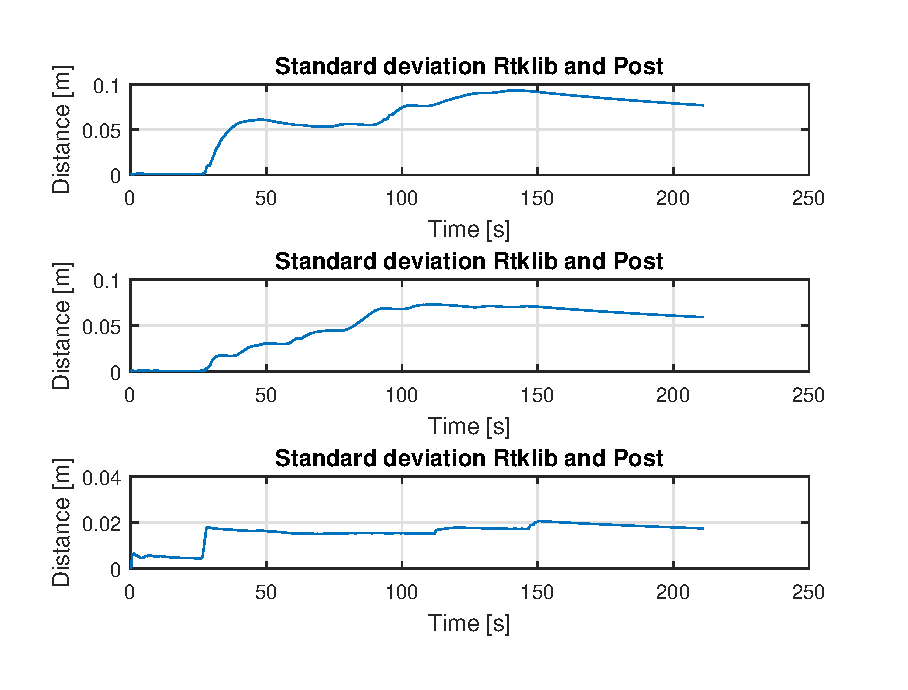
\includegraphics[width=0.7\textwidth]{figs/plots/stdrtkpost.eps}
		\caption{Standard deviation of the difference between rtklib real time and post processed solution}
		\label{figure:stdRTK}
\end{figure}
\begin{figure}[H]
	\centering
		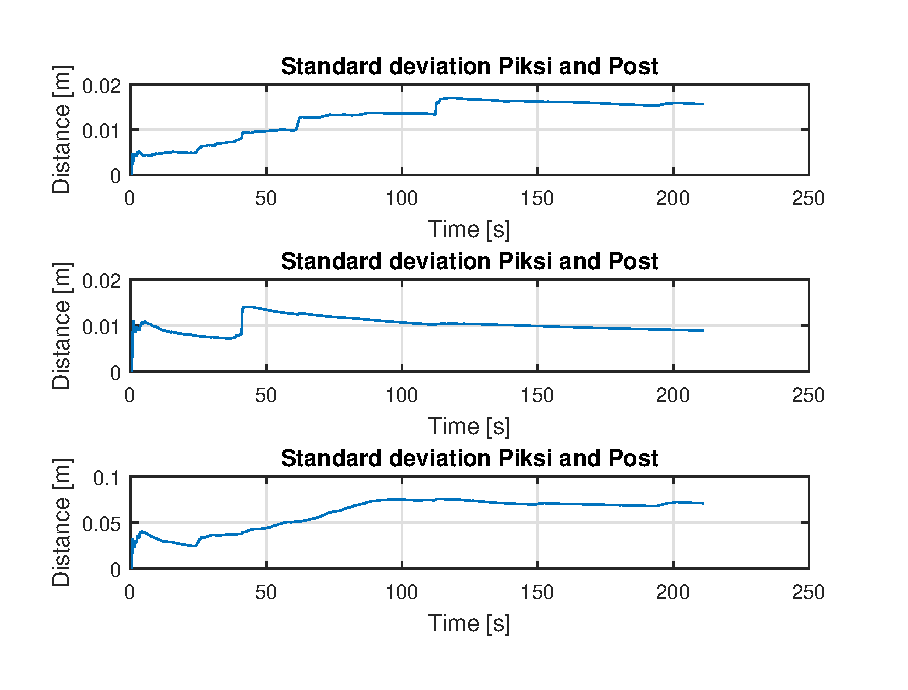
\includegraphics[width=0.7\textwidth]{figs/plots/stdpiksipost.eps}
		\caption{Standard deviation of the difference between piksi real time and rtklib post processed solution}
		\label{figure:stdPiksi}
\end{figure}
Both the Piksi and \gls{rtklib} appear to be able to correctly estimate the North and East velocity, as seen in figure \ref{figure:VelocityWalk1}. However the Down velocity from \gls{rtklib} is more noisy then the Piksi.
\begin{figure}[H]
	\centering
		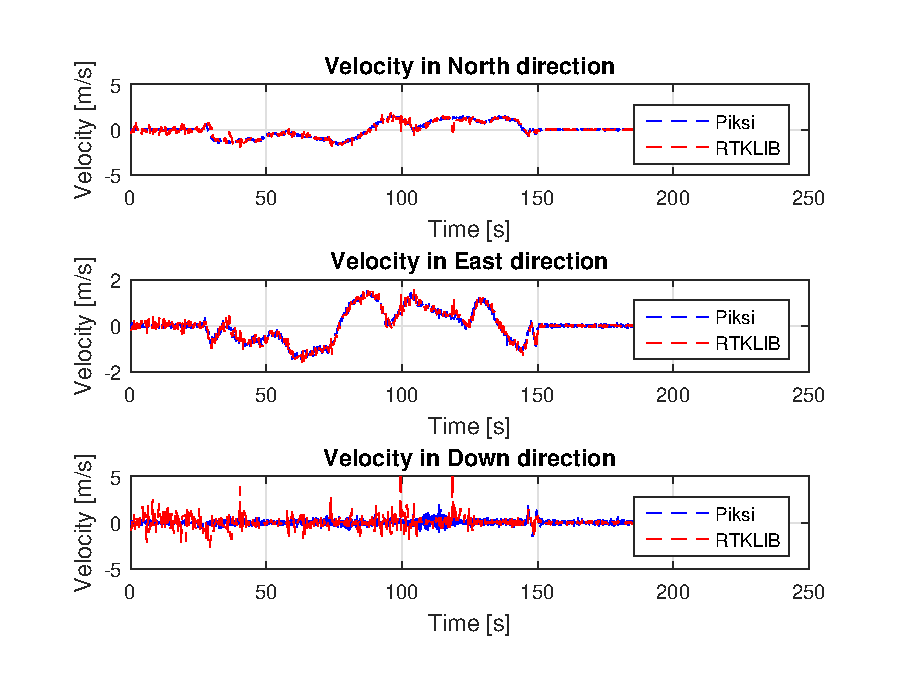
\includegraphics[width=0.7\textwidth]{figs/plots/velocityWalk1.eps}
		\caption{Velocity data from the piksi and rtklib real time solution}
		\label{figure:VelocityWalk1}
\end{figure}
%The problem with the \gls{tow} is shown more clearly in figure \ref{figure:timeRTKwalk1}. The figure display the time difference between each output. The first part is an altered version of the \gls{tow} from rtklib, while the other is the timestamp of the same output given by Dune. The output from rtklib gave only seconds, and not a millisecond value. To correct for this error the \gls{tow} value from rtklib altered to fill the gap between each second. The alteration was done by counting the number of elements with the same \gls{tow} value, and then equally spread them from between the \gls{tow} value to the next \gls{tow} value.
%
%The timestamp given by Dune indicate the delay a output message from rtklib might experience before it's available for consumption. Both the timestamp and \gls{tow} value indicate that rtklib has a mean output of 5 Hz. Here it should be noted that the ublox was configured with a output rate of 10 Hz.
%\begin{figure}[H]
%	\centering
%		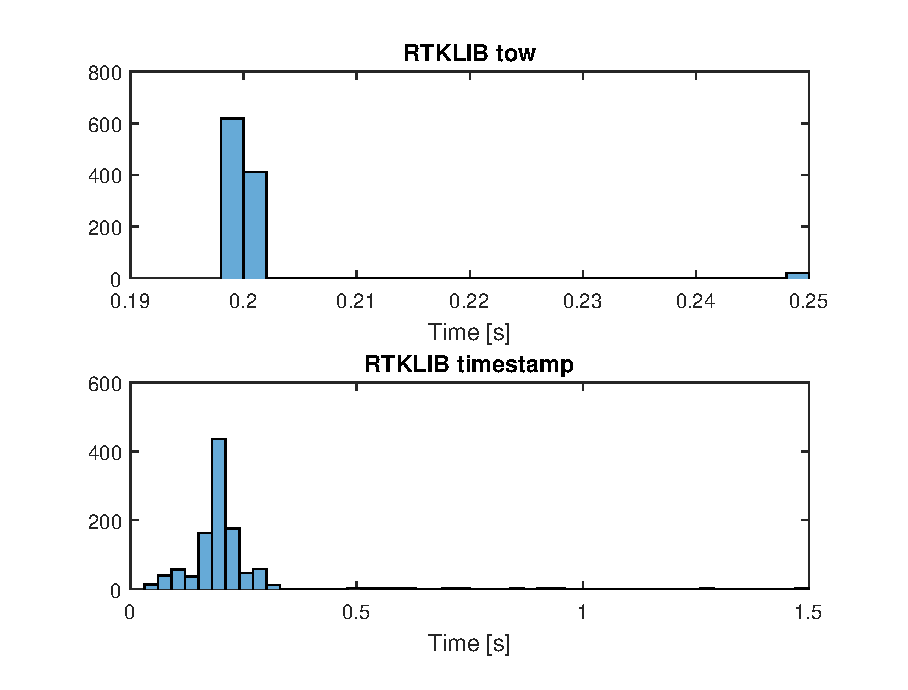
\includegraphics[width=0.7\textwidth]{figs/plots/rtktime.eps}
%		\caption{The time between time samples from rtklib}
%		\label{figure:timeRTKwalk1}
%\end{figure}
%Figure \ref{figure:timePiksiWalk1} shows the time difference between each output sample. The first plot shows the difference between each \gls{tow} value from Piksi, and the other the difference between each time stamp given by Dune. Both plots indicate that Piksi is able to have a output frequency at 10 Hz.
%\begin{figure}[H]
%	\centering
%		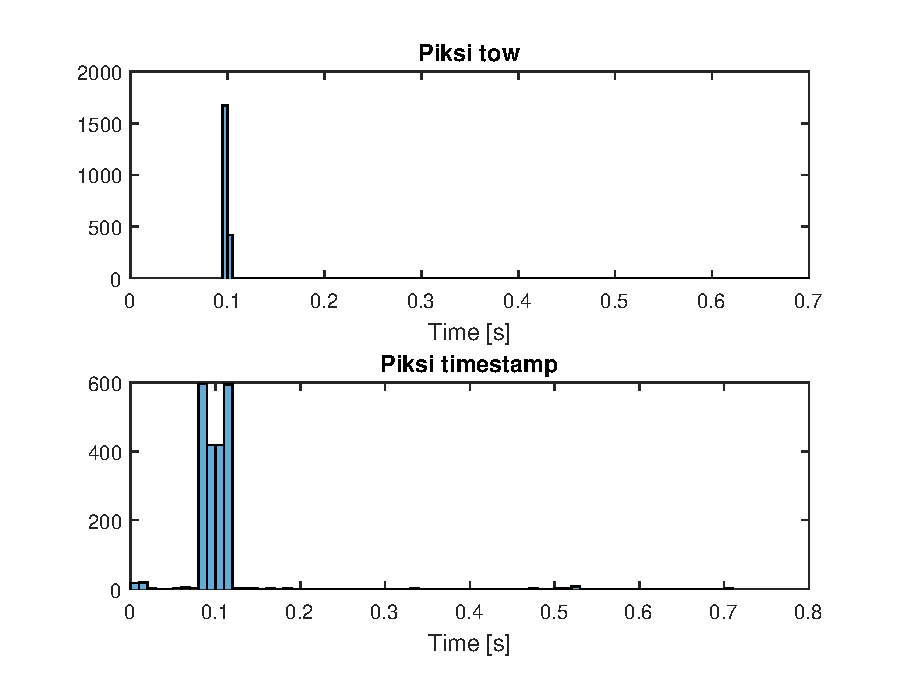
\includegraphics[width=0.7\textwidth]{figs/plots/piksitime.eps}
%		\caption{The time between time samples from rtklib}
%		\label{figure:timePiksiWalk1}
%\end{figure}
The different receiver used in Rtklib and Piksi was not able to track the same satellites at all time. Figure \ref{figure:NumSatWalk1} shows that the Ublox LEA M8T receiver connected to Rtklib managed to track more satellite then the receiver used in Piksi.
Figure 
\begin{figure}[H]
	\centering
		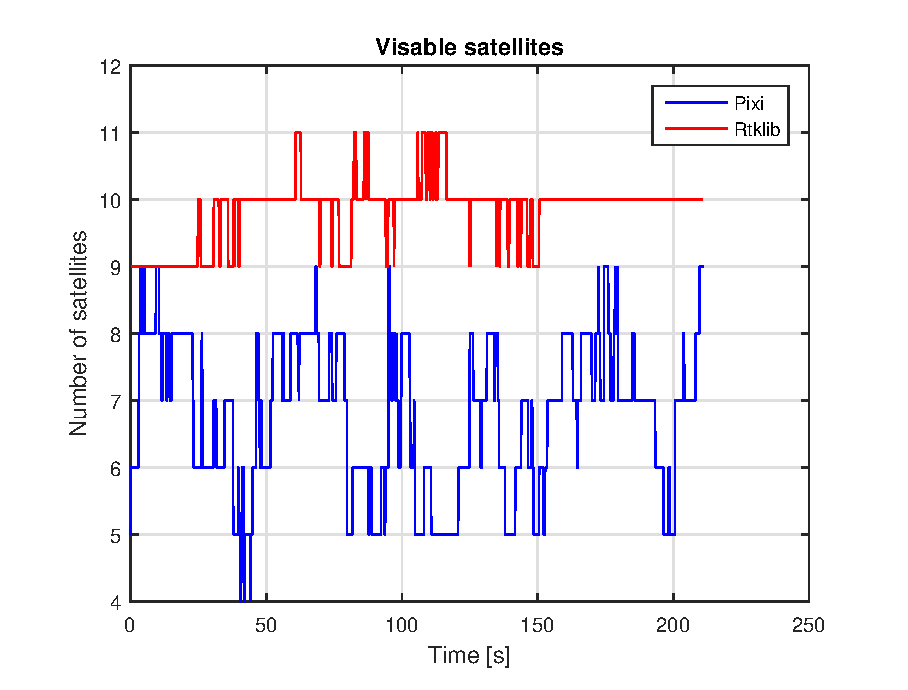
\includegraphics[width=0.7\textwidth]{figs/plots/sv.eps}
		\caption{Visable statellite for the piksi and rtklib}
		\label{figure:NumSatWalk1}
\end{figure}
The position estimate of the rover is a relative position in reference to the base station. Due to the fact that the position of the base station is calculated with a single receiver with one frequency, there will be introduced a bias in the position estimate. Figure \ref{figure:enhancedxywalk1} shows the North, East position of the the first walk. The true position is exactly the same, but in the figure it appear that the distance is approximately $5cm$. The distance from the base station to the estimated start and stop position was calculated to be $3.29m$ and $3.26$ respectfully. The measured distance was approximately $3.3m$. That gives an initial error off $0.04m$. This gives an accuracy level at centimeter level at stationary condition. 
\begin{figure}[H]
	\centering
		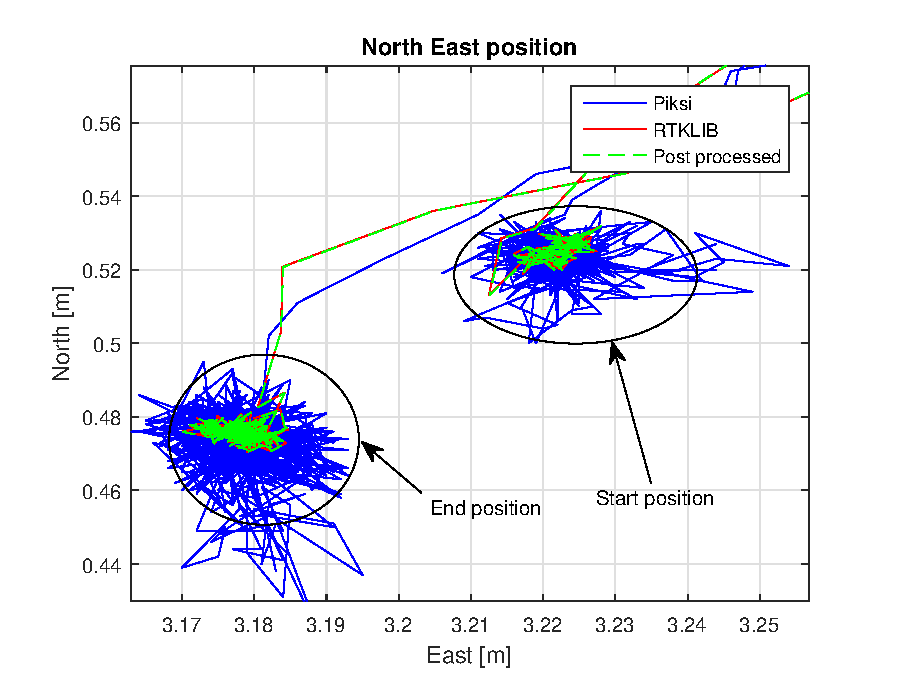
\includegraphics[width=0.7\textwidth]{figs/plots/enhancedxywalk1.eps}
		\caption{Visable statellite for the piksi and rtklib}
		\label{figure:enhancedxywalk1}
\end{figure}
The position estimate from \gls{rtklib} appear to be delay in comparison to the solution from the Piksi. Figure \ref{figure:DownDelay} shows that both the post processed solution and the real time solution is delay by $0.5$ secounds compared to the Piksi. This could be how \gls{rtklib} resolve the millisecond in \acrfull{tow}, and will not be seen as an extra delay seen from the control systems perspective.
\begin{figure}[H]
	\centering
		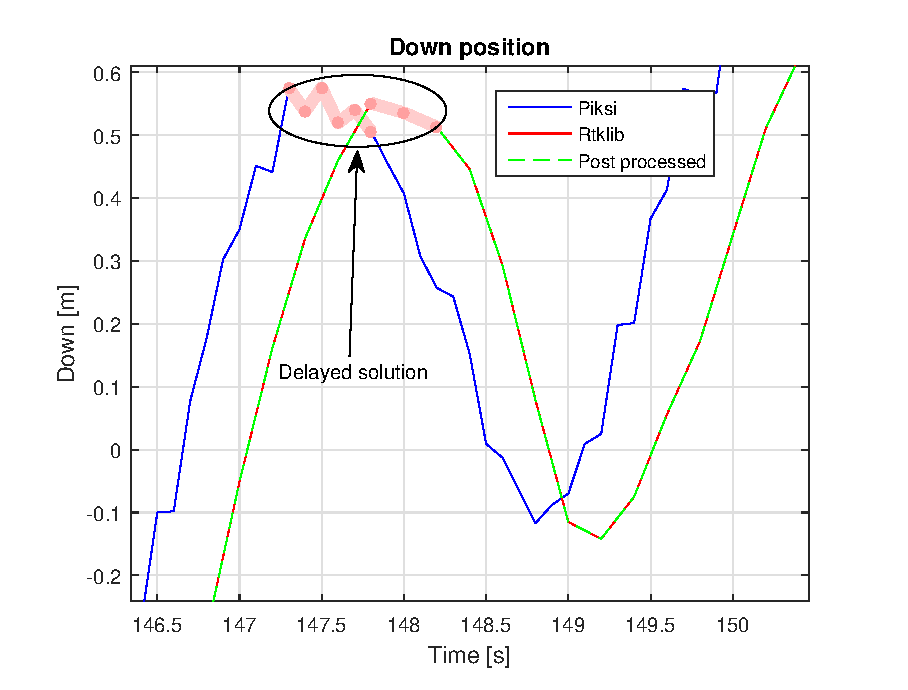
\includegraphics[width=0.7\textwidth]{figs/plots/downDelay.eps}
		\caption{Velocity data from the piksi and rtklib real time solution}
		\label{figure:DownDelay}
\end{figure}
Given that the error given in figure \ref{figure:errorPiksiwalk1} and \ref{figure:errorRTKwalk1} is never has a greater absolute value then $0.2m$ it's possible to assume that the true error will be bellow $1m$ which was given as an evasion criterion in the MSc thesis by \citep{Froelich}, if the \gls{rtk-gps} system has a fixed integer solution.

\subsubsection{Second session}
The second session was perform few minutes after the first, whit the same weather condition.
During the second session the Piksi lost its fixed integer solution, while Rtklib managed to keep its fixed integer solution as seen in figure \ref{figure:xyWalk2} and \ref{figure:downWalk2}. 
\begin{figure}[H]
	\centering
		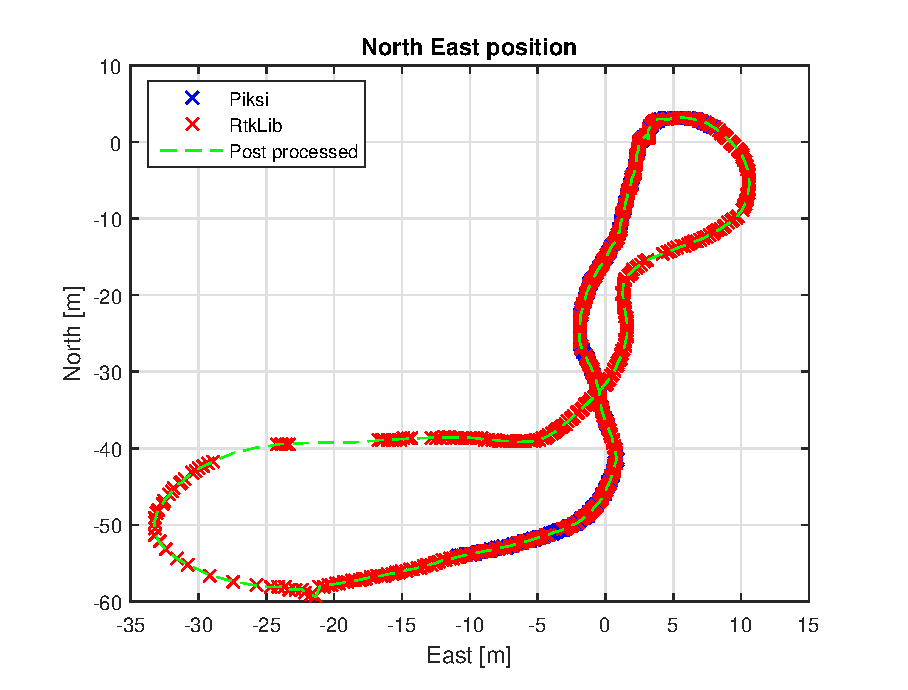
\includegraphics[width=0.7\textwidth]{figs/plots/xywalk2.eps}
		\caption{Visable statellite for the piksi and rtklib}
		\label{figure:xyWalk2}
\end{figure}
\begin{figure}[H]
	\centering
		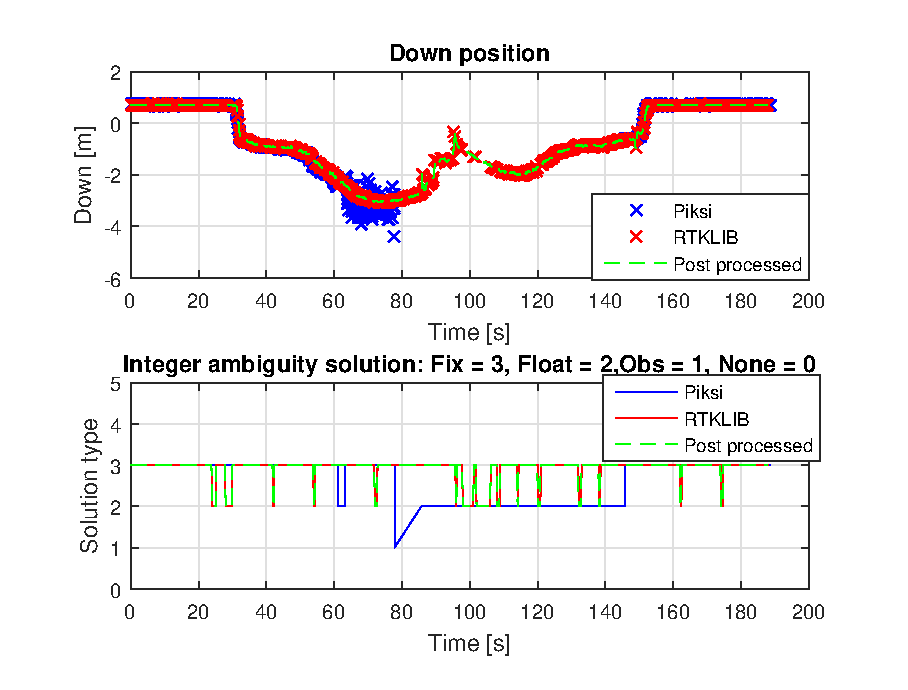
\includegraphics[width=0.7\textwidth]{figs/plots/downWalk2.eps}
		\caption{Visable statellite for the piksi and rtklib}
		\label{figure:downWalk2}
\end{figure}
The reason for why the Piksi lost its fixed solution might be because it lost track of several satellite, as seen in figure \ref{figure:numSatWalk2}. Since both receive share the same antenna it can be concluded that the satellite tracing performance in the Ublox is superior to the Piksi.  Even when the Piksi managed to regain track of the satellite it lost, it took 60 seconds before it regain a fixed integer solution. 
\begin{figure}[H]
	\centering
		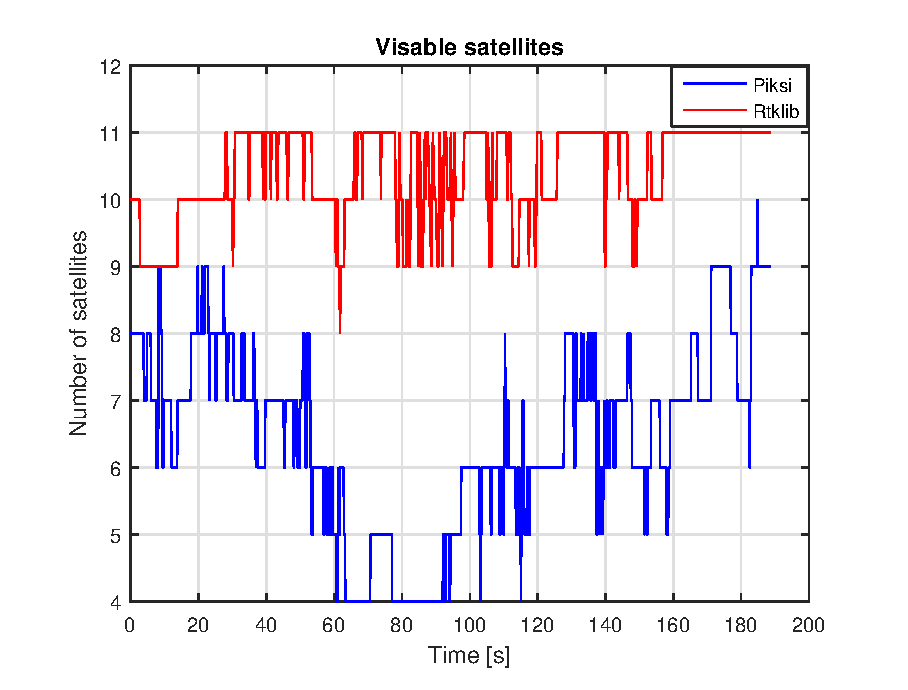
\includegraphics[width=0.7\textwidth]{figs/plots/numSatWalk2.eps}
		\caption{Visable statellite for the piksi and rtklib}
		\label{figure:numSatWalk2}
\end{figure}
\subsection{In-flight test}
A flight test with the \gls{uav} was performed at Udduvoll. Because of bad weather the were only performed one flight, and before the flight started only the Rtklib had a fixed solution. That is why in this part only performance from the Rtklib is considered, as a fixed solution is a must for a automatic landing system. 

During the flight test the integer ambiguity solution were more float then fixed as seen in figure \ref{figure:DownFlight} and \ref{figure:northEastFlight}, which affected the measurement. The same behavior will be seen during the landing, however if the float solution is accurate enough the system should be able to perform a automatic landing.
\begin{figure}[H]
	\centering
		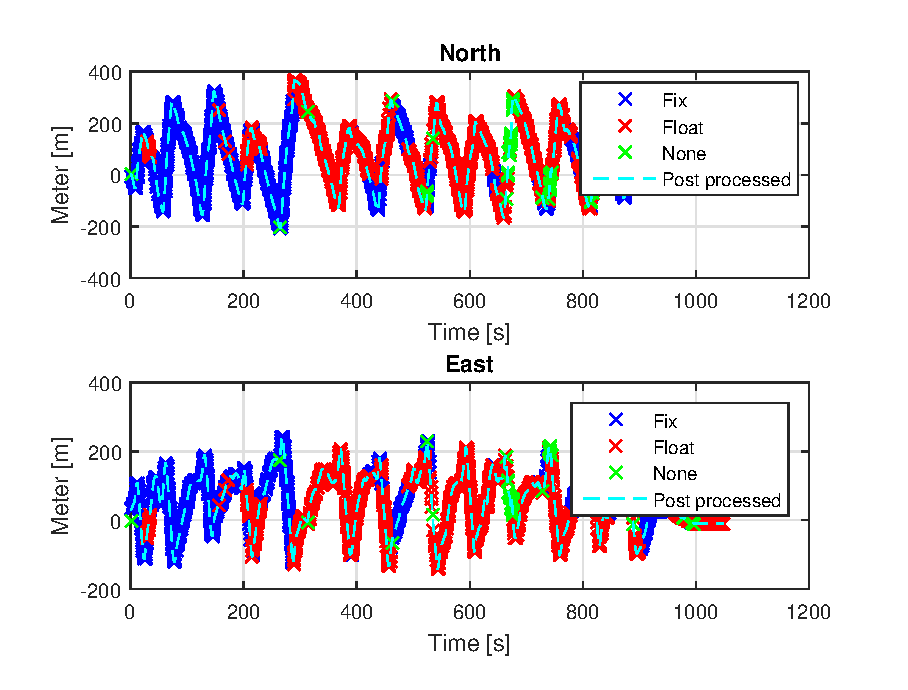
\includegraphics[width=0.7\textwidth]{figs/plots/northEastFlight.eps}
		\caption{Velocity data from the piksi and rtklib real time solution}
		\label{figure:northEastFlight}
\end{figure}
\begin{figure}[H]
	\centering
		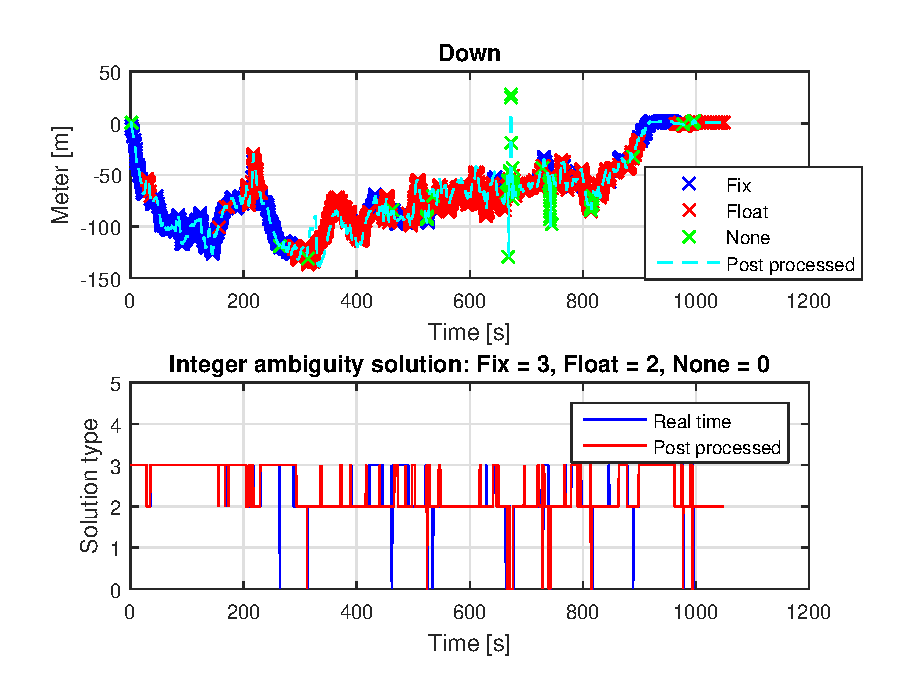
\includegraphics[width=0.7\textwidth]{figs/plots/downFlight.eps}
		\caption{Velocity data from the piksi and rtklib real time solution}
		\label{figure:DownFlight}
\end{figure}
The main reason for this behaviour is because of the number of valid satellite the receiver can track experience large variation, as seen i figure \ref{figure:numSatFlight}. A problem that was experienced during the flight is that the dynamic behaviour of the \gls{uav} blocks the antennas view of different satellites. That is a problem that can be solved by setting restricion on the dynamical behavior of the \gls{uav} expesially befor and during landing.
\begin{figure}[H]
	\centering
		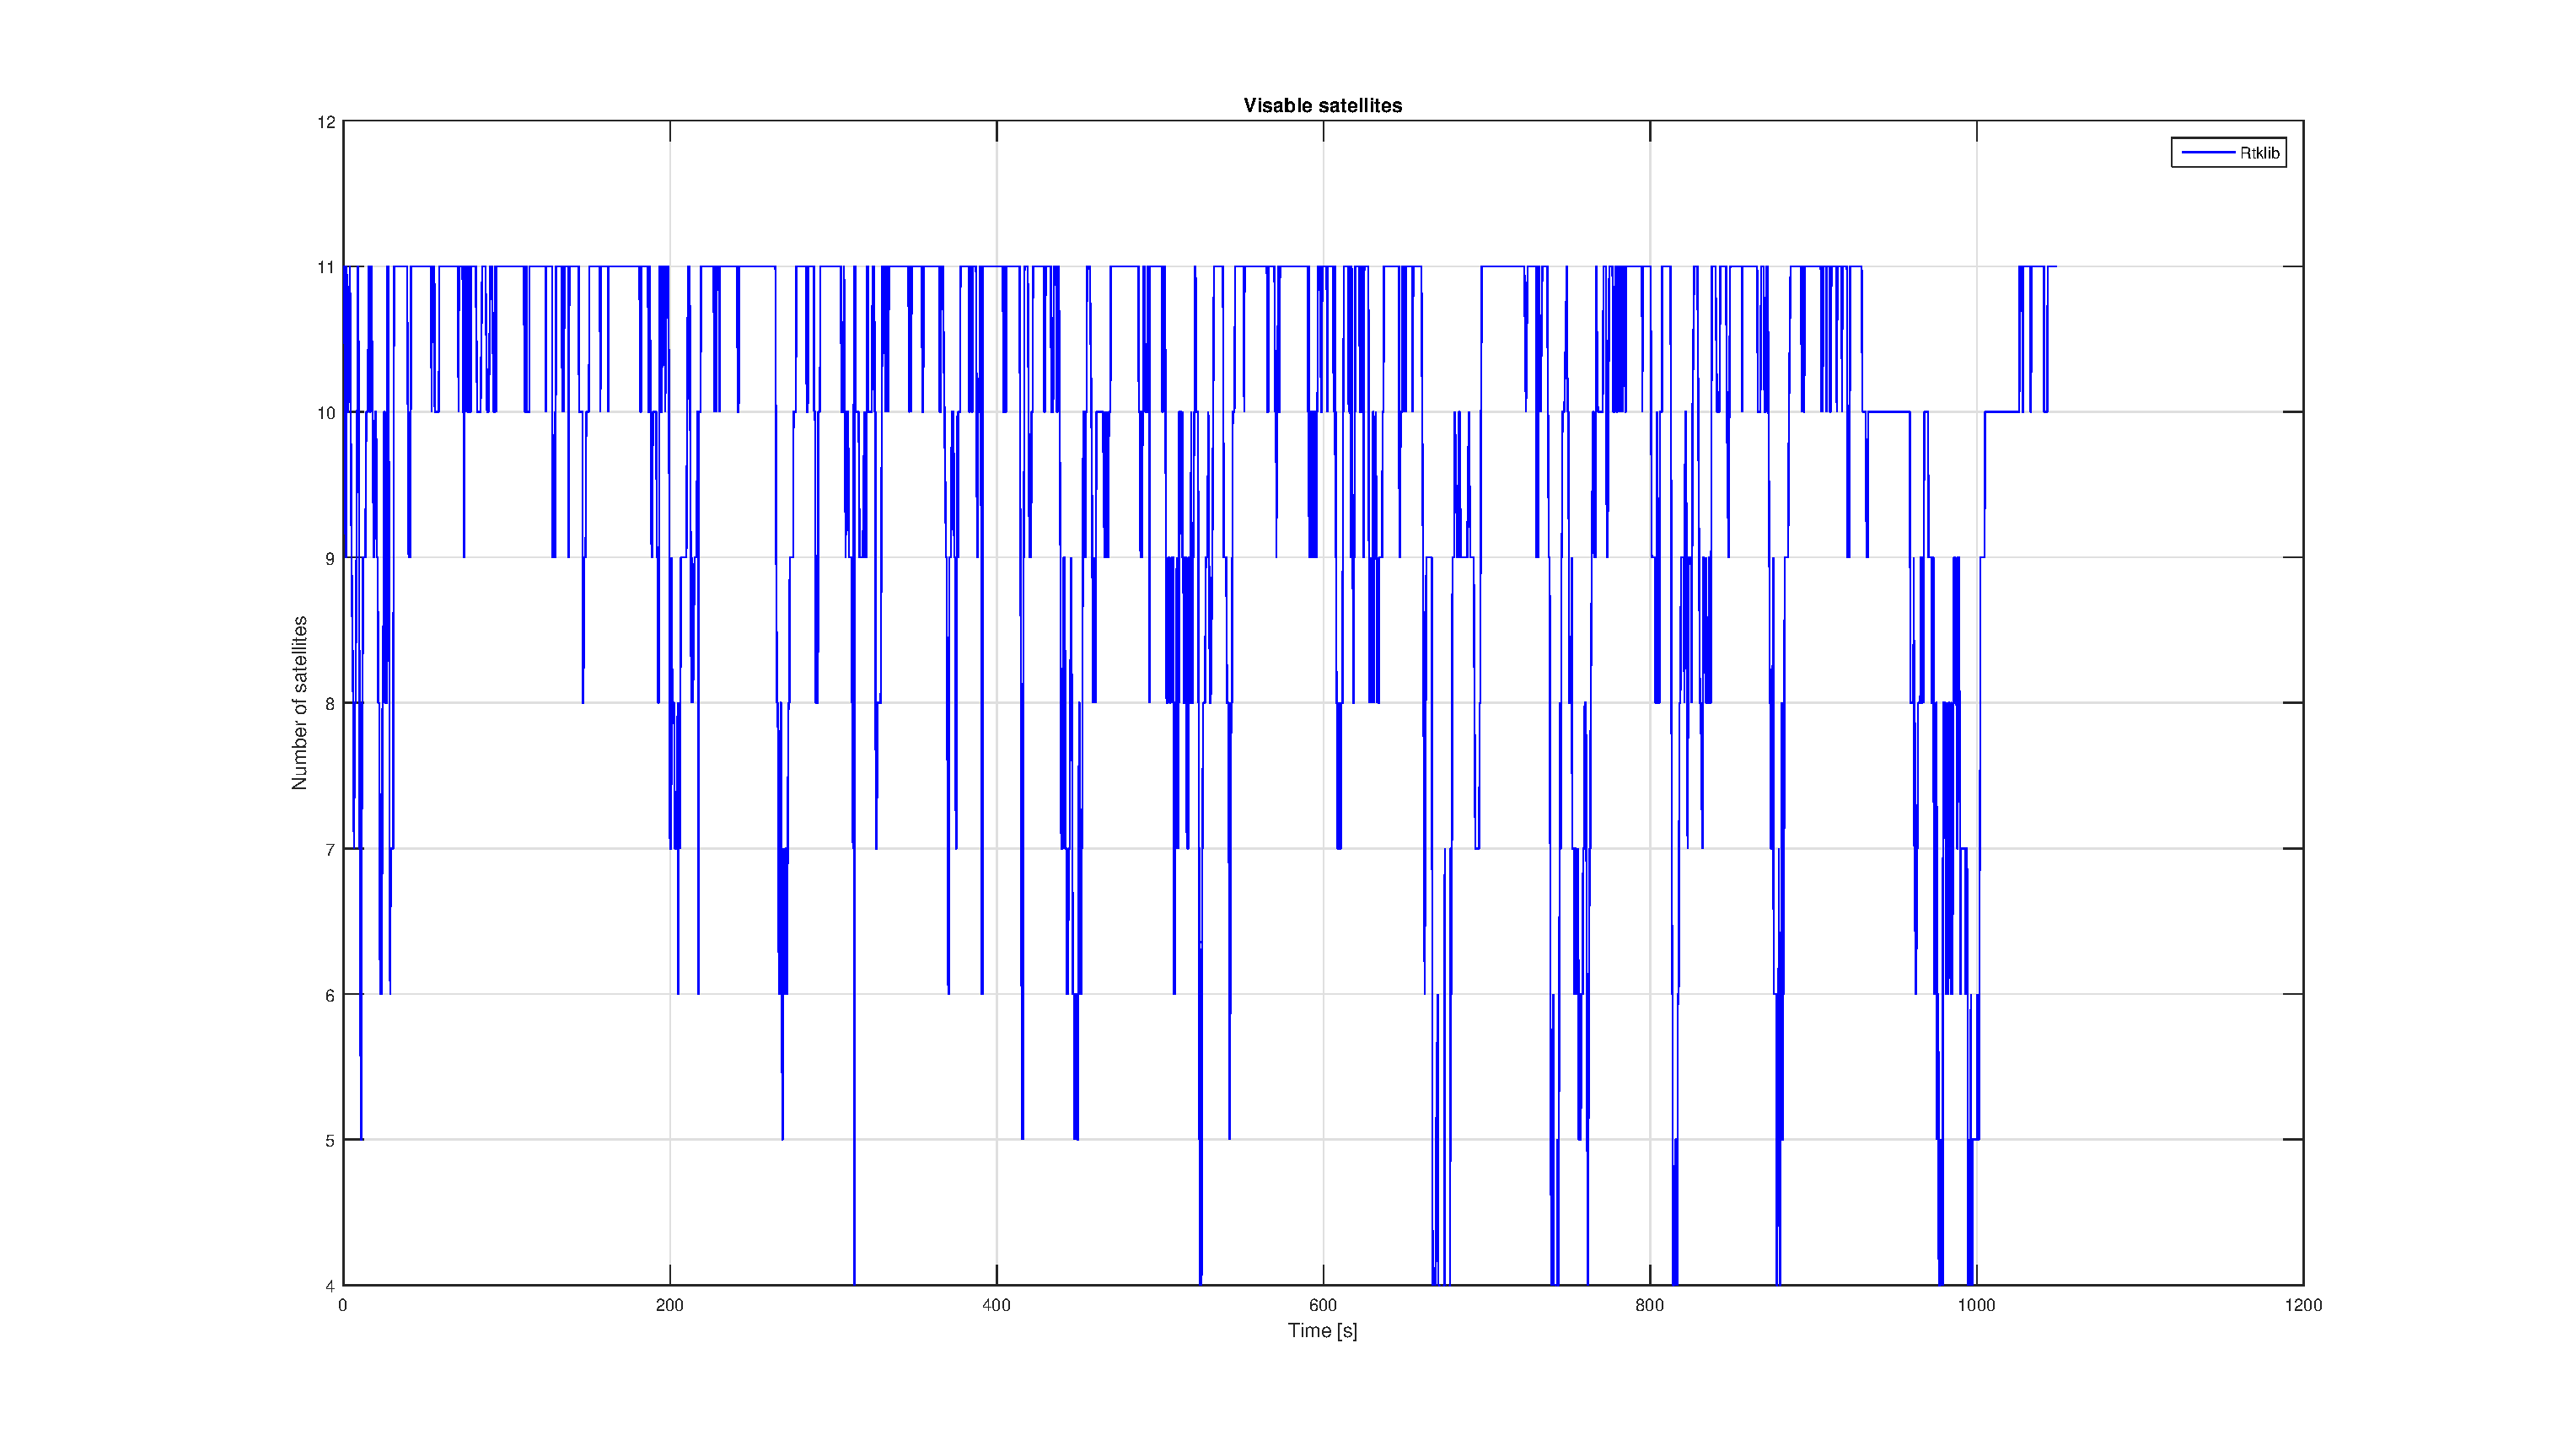
\includegraphics[width=0.7\textwidth]{figs/plots/numSatFlight.eps}
		\caption{Velocity data from the piksi and rtklib real time solution}
		\label{figure:numSatFlight}
\end{figure}
%\begin{figure}[H]
%	\centering
%		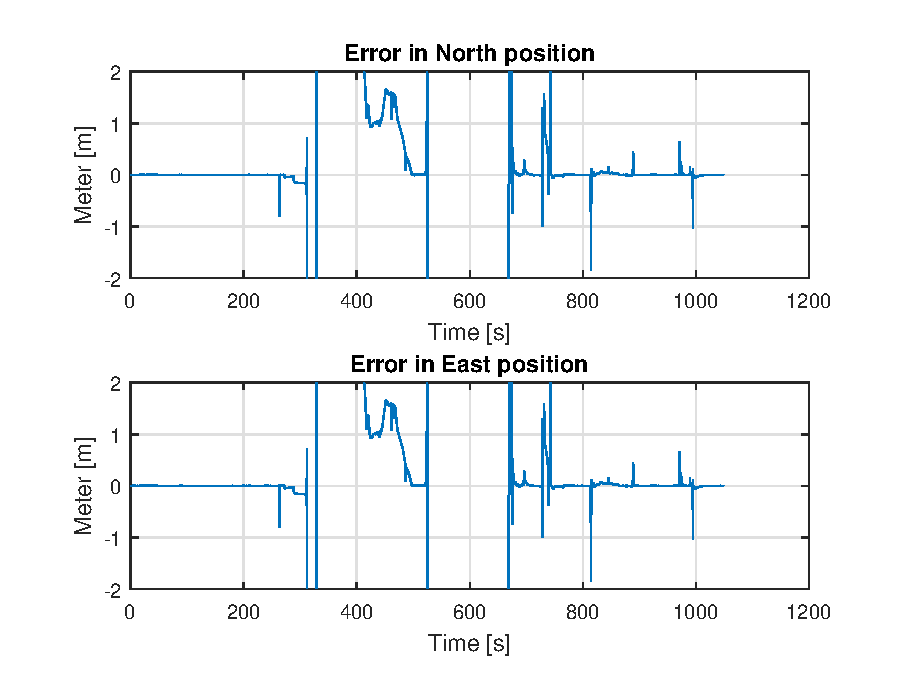
\includegraphics[width=0.7\textwidth]{figs/plots/errorNorthEastFlight.eps}
%		\caption{Velocity data from the piksi and rtklib real time solution}
%		\label{figure:errorNorthEastFlight}
%\end{figure}
%\begin{figure}[H]
%	\centering
%		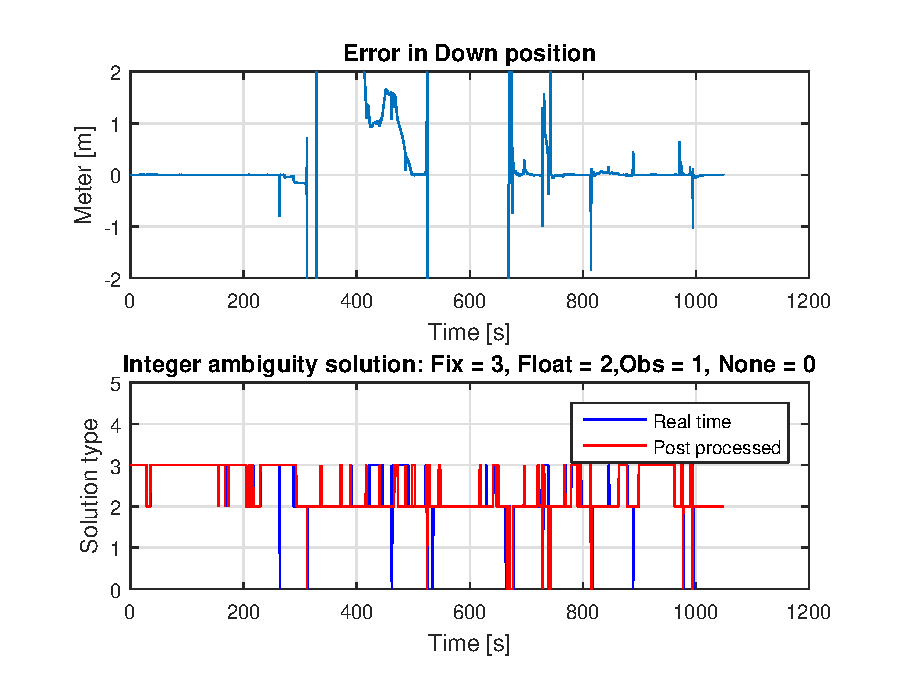
\includegraphics[width=0.7\textwidth]{figs/plots/errorDownFlight.eps}
%		\caption{Velocity data from the piksi and rtklib real time solution}
%		\label{figure:errorDownFlight}
%\end{figure}
\subsubsection{Landing}
As expected the \gls{rtk-gps} system had problem with keeping it's fixed integer solution. The \gls{rtk-gps} position estimate of the landing path is shown in figure \ref{figure:landingNEDFlight}. The system kept changing between float and fixed solution during the landing phase. Figure \ref{figure:landingNorthEastFlight} shown the North East position during the landing with the type of solution. The Down position as well as the integer ambiguity solution is for the landing phase is seen in \ref{figure:landingDownFlight}. The \gls{rtk-gps} system was unable to maintain a fixed solution, however it did maintain a float solution. Further test with a control system is required in order to test if also the float solution is accurate enough to perform a automatic landing.
\begin{figure}[H]
	\centering
		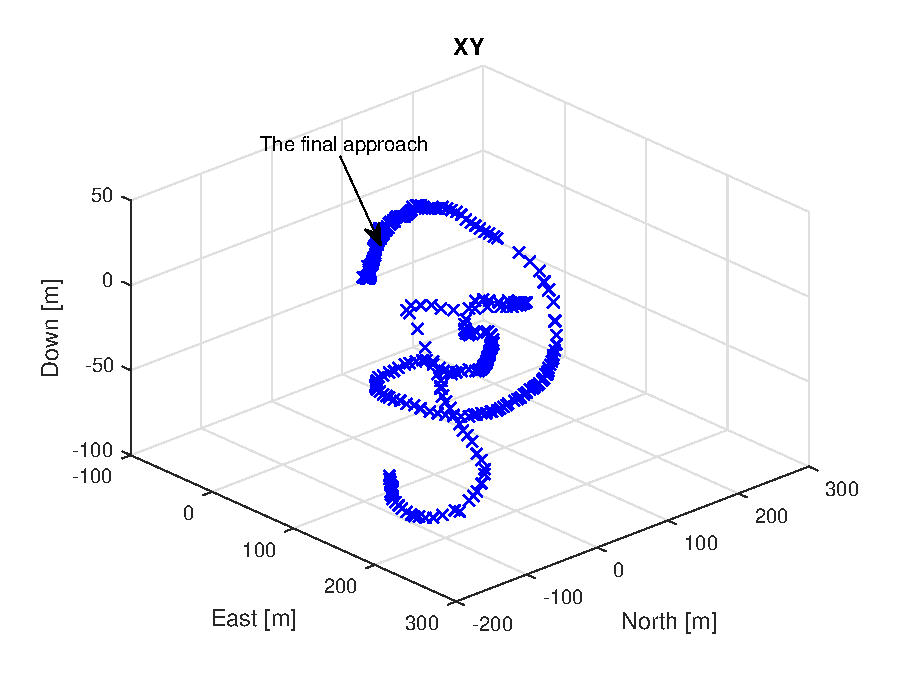
\includegraphics[width=0.7\textwidth]{figs/plots/landingNedFlight.eps}
		\caption{Velocity data from the piksi and rtklib real time solution}
		\label{figure:landingNEDFlight}
\end{figure}
\begin{figure}[H]
	\centering
		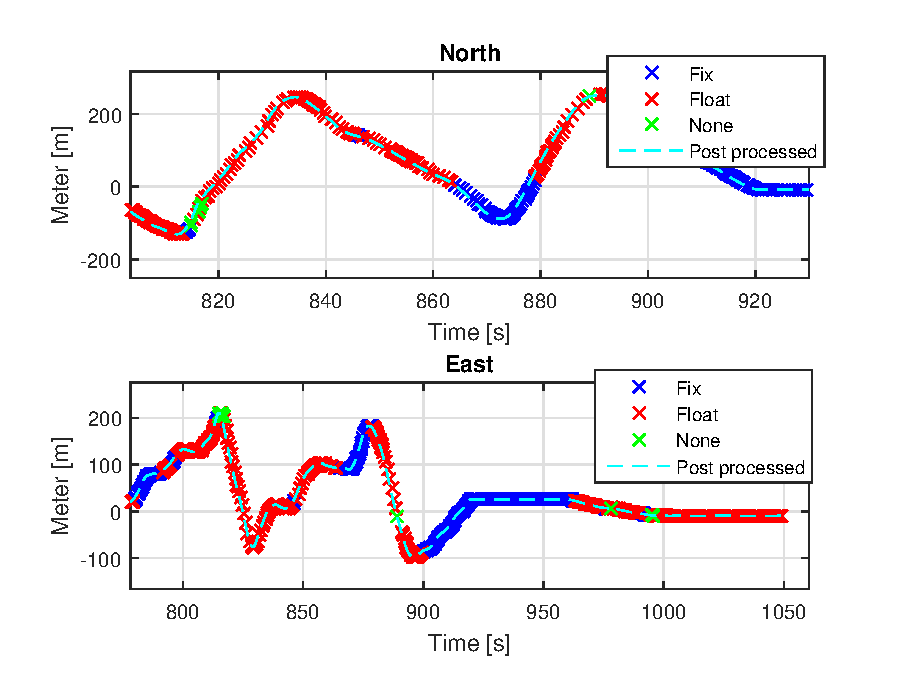
\includegraphics[width=0.7\textwidth]{figs/plots/landingNorthEastFlight.eps}
		\caption{Velocity data from the piksi and rtklib real time solution}
		\label{figure:landingNorthEastFlight}
\end{figure}
\begin{figure}[H]
	\centering
		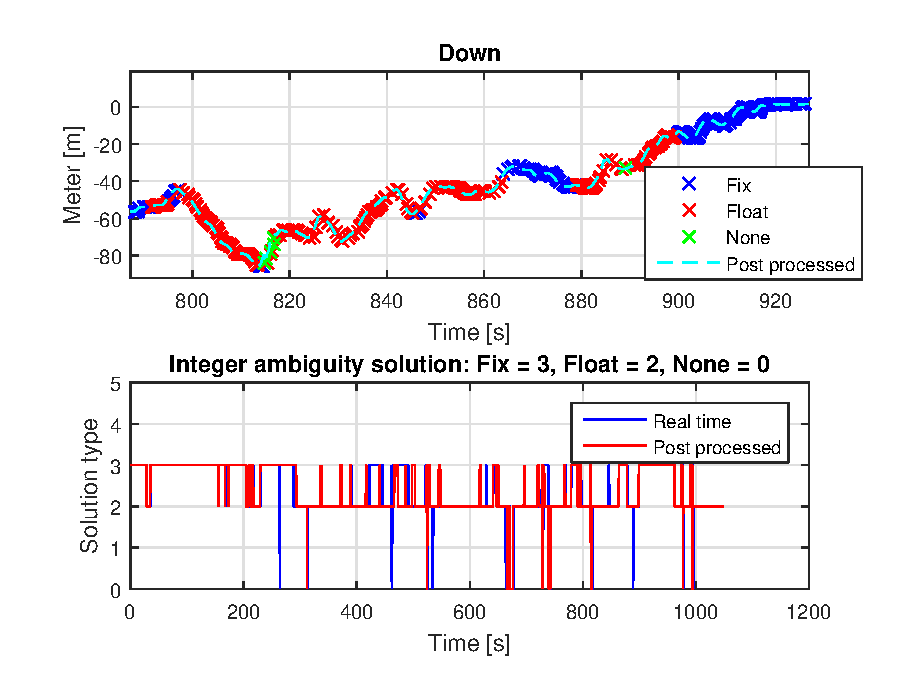
\includegraphics[width=0.7\textwidth]{figs/plots/landingDownFlight.eps}
		\caption{Velocity data from the piksi and rtklib real time solution}
		\label{figure:landingDownFlight}
\end{figure}

From the error plot seen in figure \ref{figure:landingErrorNorthEastDownFlight} it appear that to be able to estimate it's own position with an error bellow 1 meter most of the time. However this is compared to the post processed estimate, which also will diverge from the true value.

\begin{figure}[H]
	\centering
		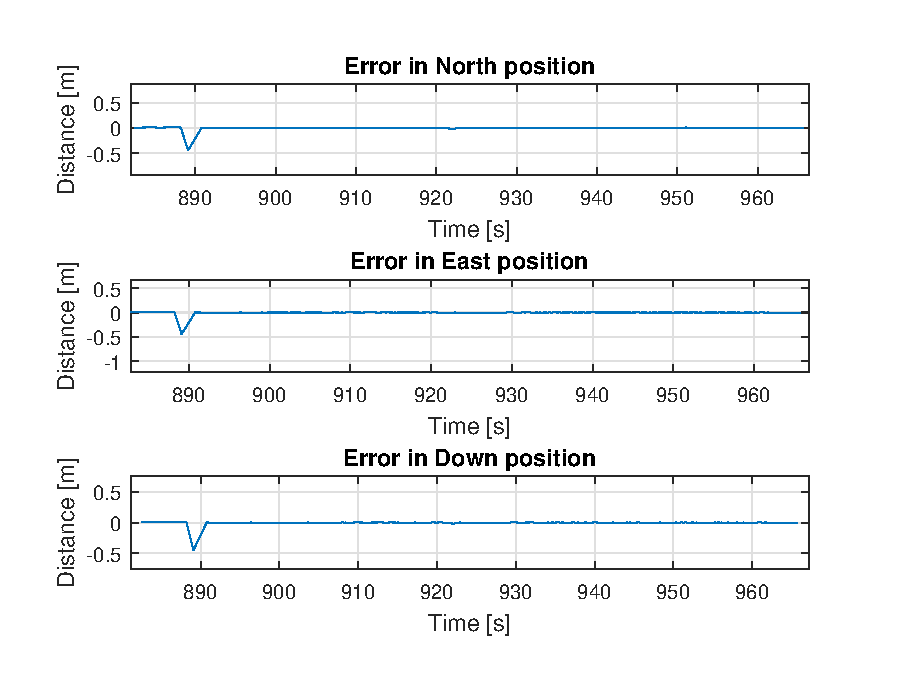
\includegraphics[width=0.7\textwidth]{figs/plots/landingErrorNorthEastDownFlight.eps}
		\caption{Velocity data from the piksi and rtklib real time solution}
		\label{figure:landingErrorNorthEastDownFlight}
\end{figure}
The landing velocity seen in \ref{figure:landingVelocity} confirms the trend see in the first session. The North and East velocity seams to get a nice estimate, however that is not the case with the Down velocity. The Down velocity estimate appear noisy, and not suited for input into a control system. 
\begin{figure}[H]
	\centering
		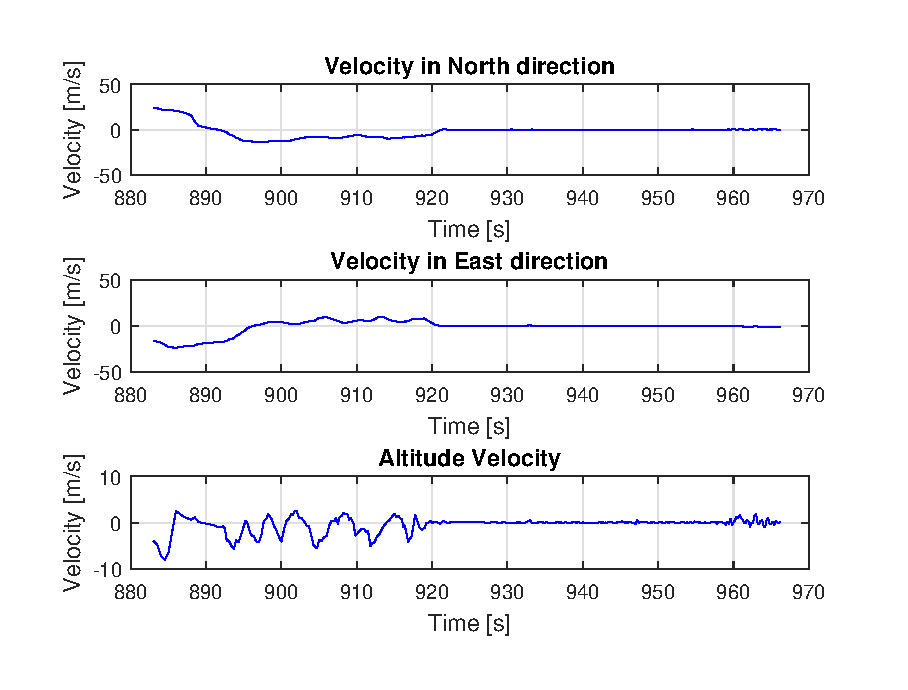
\includegraphics[width=0.7\textwidth]{figs/plots/landingVelocity.eps}
		\caption{Velocity data from the piksi and rtklib real time solution}
		\label{figure:landingVelocity}
\end{figure}
\cleardoublepage
%===================================== CHAP 5 =================================

\chapter{Conclusion and recommendation for further work}
This chapter will discus the result from the field tests, which will be used to conclude the performance of the individual \gls{rtk-gps} system. The last part of this chapter will include suggestion for further work regarding the design of a automatic net landing system.
\section{RTK-GPS lab testing}
It was seen in the lab testing that both the Piksi and \gls{rtklib} was able to get a fixed solution, although the \gls{rtklib} was faster. In the first test were the \gls{uav} was carried both system gave similar result during the first session \gls{uav}, however during the second the Piksi lost its fixed solution. Rtklib had also problem during this session, but unlike the Piksi managed to find a fixed solution again. The ability for the navigation system to quickly recover its integer solution is critical for a automatic net landing system.

The \gls{rtk-gps} system achieves centimeter level accuracy when stationary. When the \gls{uav} is in motion this will decrease down to decimeter accuracy. This can be assumed is the behaviour for the navigation system based on the stationary accuracy test, and the high precision in the position estimate. That should be good enough in a navigation system for a automatic landing system.

The output solution from \gls{rtklib} has a \acrfull{tow} value that is constant half a second delayed compared to the Piksi. It could be that \gls{rtklib} interpolate the microseconds of the \gls{tow} value from the different satellites, such that a control system do not get a delayed position estimate. However for a integrated navigation system this pose a problem. The integration becomes more difficult when it's unclear how old the position estimate is.

The tracking performance from the two receiver type indicate that the Ublox is superior to the Piksi. It always manage to track more satellites, and managed to track them longer.
\section{RTK-GPS in-flight test}
The flight test showed that keeping the fixed integer solution during a flight is difficult, most likely because of the dynamic behaviour of the \gls{uav}. The landing phase of the \gls{uav} operation should be kept independent from the rest of the operation. Therefore landing specific constraint cannot be imposed on the \gls{uav} behaviour. In order to then get a best relative position estimate the \gls{rtk-gps} must be able to recover it's fixed integer solution as quickly as possible while the \gls{uav} is in flight.

Before the take-off the Piksi had yet solved its integer ambiguity, while \gls{rtklib} had. That might be because of it kept track of fever satellites. However the navigation system must be able to resolve its integer ambiguity quickly to increase the probability of performing a safe and successfully automatic landing.

During the flight the Ublox lost track of more satellite then during the \gls{gps} lab tests. The antenna follows the orientation of the \gls{uav} and therefore some satellite will be blocked by the fuselage. This must be consider when designing a guidance system for automatic landing. To ensure that the antenna has a clear view of the sky, the \gls{uav} should try to have a maximum roll when the automatic landing system is engaged.

The velocity estimate from Piksi and \gls{rtklib} in the first test have similar estimate for the North and East component, but differ in the Down component. In the flight test the \gls{rtklib} altitude velocity was better, such that it can be used in a control system.
%
%
%
%
%
%
%
%DO NOT INCLUDE WHAT IS BELLOW BEFORE FURTHER WORK
%
%
%It might be that the float position estimate is good enough to perform a automatic landing. Further test are required.
%
%Rtklib managed to keep float/fixed solution during the landing.
%
%The rtklib was the only system able to get a fixed solution. Discus the performance of rtklib, whit the ublox receiver. 
%
%What can be concluded:
%
%Rtklib is able to faster find a fixed solution. Can be because of better receiver, better integer ambiguity resolution strategy, poorer validation of ambiguity, more efficient algorithm. Based on how many satellites the ublox receiver manage to track I will say that the receiver had a large part in shortening the time.
%
%When fixed there is not a large deviation between the two solutions. One difference that might cause problem in a guidance system is that it appear that the solution from rtklib is delayed. The \gls{tow} that's given with the solution do not include the millisecond value. 
%
%The Piksi is faster to calculate the position, but slower to resolve the integer ambiguity. 
%
%The conclusion of the different system. Piksi has better and more efficient solution software, however rtklib can use a superior \gls{gnss} receiver.
%
%Both system has a good estimation of the North and East velocity, however it appear that rtklib has problem estimating the vertical velocity.


\section{Further work}
The Ublox receiver and the \gls{gnss} antennas are able to receive both \gls{gps} and \gls{glonass} \gls{l1} signals, which should be exploited to increase the number of valid satellite available for the \gls{rtk-gps} system. This could also give better constellation geometry, and help the system resolve its integer ambiguity faster.

The \gls{rtk-gps} system must be integrated with the existing control and guidance system, and a test landing in a stationary net must be performed. 

A \gls{rtk-gps} system can use both the Piksi and Rtklib such that the automatic landing system has redundancy in position, and velocity estimation. A validation task must then be design to choose which of the system should send the rtkfix \gls{imc} message to the rest of the system.

A \gls{rtk-gps}/gls{ins} integration navigation system can be implemented in the automatic landing system. A \gls{rtk-gps}/gls{ins} integration was proposed in \citep{Spockeli}, which can be used.

A position estimation system that can accurately predict were the \gls{uav} will be a few seconds ahead of time, such that the \gls{uav} can better know were it is instead of were if was.

Setting constraints on the path such that the antenna has a clear view of the satellites at all time during the landing phase. 
\cleardoublepage
%% include here the other chapters

\renewcommand*{\bibname}{References}
\bibliographystyle{plainnat}
\bibliography{main}

%% Uncomment the following if you have any appendix
% \appendix
% \addtocontents{toc}{%
%  \protect\vspace{1em}% 
%  \protect\noindent \bfseries \appendixtocname\protect\par
%  \protect\vspace{-.5em}%
% }
% \renewcommand{\chaptername}{\appendixname}
%% include below possible appendices (chapters)


\end{document} 
